% Options for packages loaded elsewhere
\PassOptionsToPackage{unicode}{hyperref}
\PassOptionsToPackage{hyphens}{url}
\PassOptionsToPackage{dvipsnames,svgnames,x11names}{xcolor}
%
\documentclass[
  letterpaper,
  DIV=11,
  numbers=noendperiod]{scrreprt}

\usepackage{amsmath,amssymb}
\usepackage{iftex}
\ifPDFTeX
  \usepackage[T1]{fontenc}
  \usepackage[utf8]{inputenc}
  \usepackage{textcomp} % provide euro and other symbols
\else % if luatex or xetex
  \usepackage{unicode-math}
  \defaultfontfeatures{Scale=MatchLowercase}
  \defaultfontfeatures[\rmfamily]{Ligatures=TeX,Scale=1}
\fi
\usepackage{lmodern}
\ifPDFTeX\else  
    % xetex/luatex font selection
\fi
% Use upquote if available, for straight quotes in verbatim environments
\IfFileExists{upquote.sty}{\usepackage{upquote}}{}
\IfFileExists{microtype.sty}{% use microtype if available
  \usepackage[]{microtype}
  \UseMicrotypeSet[protrusion]{basicmath} % disable protrusion for tt fonts
}{}
\makeatletter
\@ifundefined{KOMAClassName}{% if non-KOMA class
  \IfFileExists{parskip.sty}{%
    \usepackage{parskip}
  }{% else
    \setlength{\parindent}{0pt}
    \setlength{\parskip}{6pt plus 2pt minus 1pt}}
}{% if KOMA class
  \KOMAoptions{parskip=half}}
\makeatother
\usepackage{xcolor}
\setlength{\emergencystretch}{3em} % prevent overfull lines
\setcounter{secnumdepth}{5}
% Make \paragraph and \subparagraph free-standing
\ifx\paragraph\undefined\else
  \let\oldparagraph\paragraph
  \renewcommand{\paragraph}[1]{\oldparagraph{#1}\mbox{}}
\fi
\ifx\subparagraph\undefined\else
  \let\oldsubparagraph\subparagraph
  \renewcommand{\subparagraph}[1]{\oldsubparagraph{#1}\mbox{}}
\fi

\usepackage{color}
\usepackage{fancyvrb}
\newcommand{\VerbBar}{|}
\newcommand{\VERB}{\Verb[commandchars=\\\{\}]}
\DefineVerbatimEnvironment{Highlighting}{Verbatim}{commandchars=\\\{\}}
% Add ',fontsize=\small' for more characters per line
\usepackage{framed}
\definecolor{shadecolor}{RGB}{241,243,245}
\newenvironment{Shaded}{\begin{snugshade}}{\end{snugshade}}
\newcommand{\AlertTok}[1]{\textcolor[rgb]{0.68,0.00,0.00}{#1}}
\newcommand{\AnnotationTok}[1]{\textcolor[rgb]{0.37,0.37,0.37}{#1}}
\newcommand{\AttributeTok}[1]{\textcolor[rgb]{0.40,0.45,0.13}{#1}}
\newcommand{\BaseNTok}[1]{\textcolor[rgb]{0.68,0.00,0.00}{#1}}
\newcommand{\BuiltInTok}[1]{\textcolor[rgb]{0.00,0.23,0.31}{#1}}
\newcommand{\CharTok}[1]{\textcolor[rgb]{0.13,0.47,0.30}{#1}}
\newcommand{\CommentTok}[1]{\textcolor[rgb]{0.37,0.37,0.37}{#1}}
\newcommand{\CommentVarTok}[1]{\textcolor[rgb]{0.37,0.37,0.37}{\textit{#1}}}
\newcommand{\ConstantTok}[1]{\textcolor[rgb]{0.56,0.35,0.01}{#1}}
\newcommand{\ControlFlowTok}[1]{\textcolor[rgb]{0.00,0.23,0.31}{#1}}
\newcommand{\DataTypeTok}[1]{\textcolor[rgb]{0.68,0.00,0.00}{#1}}
\newcommand{\DecValTok}[1]{\textcolor[rgb]{0.68,0.00,0.00}{#1}}
\newcommand{\DocumentationTok}[1]{\textcolor[rgb]{0.37,0.37,0.37}{\textit{#1}}}
\newcommand{\ErrorTok}[1]{\textcolor[rgb]{0.68,0.00,0.00}{#1}}
\newcommand{\ExtensionTok}[1]{\textcolor[rgb]{0.00,0.23,0.31}{#1}}
\newcommand{\FloatTok}[1]{\textcolor[rgb]{0.68,0.00,0.00}{#1}}
\newcommand{\FunctionTok}[1]{\textcolor[rgb]{0.28,0.35,0.67}{#1}}
\newcommand{\ImportTok}[1]{\textcolor[rgb]{0.00,0.46,0.62}{#1}}
\newcommand{\InformationTok}[1]{\textcolor[rgb]{0.37,0.37,0.37}{#1}}
\newcommand{\KeywordTok}[1]{\textcolor[rgb]{0.00,0.23,0.31}{#1}}
\newcommand{\NormalTok}[1]{\textcolor[rgb]{0.00,0.23,0.31}{#1}}
\newcommand{\OperatorTok}[1]{\textcolor[rgb]{0.37,0.37,0.37}{#1}}
\newcommand{\OtherTok}[1]{\textcolor[rgb]{0.00,0.23,0.31}{#1}}
\newcommand{\PreprocessorTok}[1]{\textcolor[rgb]{0.68,0.00,0.00}{#1}}
\newcommand{\RegionMarkerTok}[1]{\textcolor[rgb]{0.00,0.23,0.31}{#1}}
\newcommand{\SpecialCharTok}[1]{\textcolor[rgb]{0.37,0.37,0.37}{#1}}
\newcommand{\SpecialStringTok}[1]{\textcolor[rgb]{0.13,0.47,0.30}{#1}}
\newcommand{\StringTok}[1]{\textcolor[rgb]{0.13,0.47,0.30}{#1}}
\newcommand{\VariableTok}[1]{\textcolor[rgb]{0.07,0.07,0.07}{#1}}
\newcommand{\VerbatimStringTok}[1]{\textcolor[rgb]{0.13,0.47,0.30}{#1}}
\newcommand{\WarningTok}[1]{\textcolor[rgb]{0.37,0.37,0.37}{\textit{#1}}}

\providecommand{\tightlist}{%
  \setlength{\itemsep}{0pt}\setlength{\parskip}{0pt}}\usepackage{longtable,booktabs,array}
\usepackage{calc} % for calculating minipage widths
% Correct order of tables after \paragraph or \subparagraph
\usepackage{etoolbox}
\makeatletter
\patchcmd\longtable{\par}{\if@noskipsec\mbox{}\fi\par}{}{}
\makeatother
% Allow footnotes in longtable head/foot
\IfFileExists{footnotehyper.sty}{\usepackage{footnotehyper}}{\usepackage{footnote}}
\makesavenoteenv{longtable}
\usepackage{graphicx}
\makeatletter
\def\maxwidth{\ifdim\Gin@nat@width>\linewidth\linewidth\else\Gin@nat@width\fi}
\def\maxheight{\ifdim\Gin@nat@height>\textheight\textheight\else\Gin@nat@height\fi}
\makeatother
% Scale images if necessary, so that they will not overflow the page
% margins by default, and it is still possible to overwrite the defaults
% using explicit options in \includegraphics[width, height, ...]{}
\setkeys{Gin}{width=\maxwidth,height=\maxheight,keepaspectratio}
% Set default figure placement to htbp
\makeatletter
\def\fps@figure{htbp}
\makeatother

\KOMAoption{captions}{tableheading}
\makeatletter
\makeatother
\makeatletter
\@ifpackageloaded{bookmark}{}{\usepackage{bookmark}}
\makeatother
\makeatletter
\@ifpackageloaded{caption}{}{\usepackage{caption}}
\AtBeginDocument{%
\ifdefined\contentsname
  \renewcommand*\contentsname{Table of contents}
\else
  \newcommand\contentsname{Table of contents}
\fi
\ifdefined\listfigurename
  \renewcommand*\listfigurename{List of Figures}
\else
  \newcommand\listfigurename{List of Figures}
\fi
\ifdefined\listtablename
  \renewcommand*\listtablename{List of Tables}
\else
  \newcommand\listtablename{List of Tables}
\fi
\ifdefined\figurename
  \renewcommand*\figurename{Figure}
\else
  \newcommand\figurename{Figure}
\fi
\ifdefined\tablename
  \renewcommand*\tablename{Table}
\else
  \newcommand\tablename{Table}
\fi
}
\@ifpackageloaded{float}{}{\usepackage{float}}
\floatstyle{ruled}
\@ifundefined{c@chapter}{\newfloat{codelisting}{h}{lop}}{\newfloat{codelisting}{h}{lop}[chapter]}
\floatname{codelisting}{Listing}
\newcommand*\listoflistings{\listof{codelisting}{List of Listings}}
\makeatother
\makeatletter
\@ifpackageloaded{caption}{}{\usepackage{caption}}
\@ifpackageloaded{subcaption}{}{\usepackage{subcaption}}
\makeatother
\makeatletter
\@ifpackageloaded{tcolorbox}{}{\usepackage[skins,breakable]{tcolorbox}}
\makeatother
\makeatletter
\@ifundefined{shadecolor}{\definecolor{shadecolor}{rgb}{.97, .97, .97}}
\makeatother
\makeatletter
\makeatother
\makeatletter
\makeatother
\ifLuaTeX
  \usepackage{selnolig}  % disable illegal ligatures
\fi
\IfFileExists{bookmark.sty}{\usepackage{bookmark}}{\usepackage{hyperref}}
\IfFileExists{xurl.sty}{\usepackage{xurl}}{} % add URL line breaks if available
\urlstyle{same} % disable monospaced font for URLs
\hypersetup{
  pdftitle={ISLR-R21.\_1},
  pdfauthor={Norah Jones},
  colorlinks=true,
  linkcolor={blue},
  filecolor={Maroon},
  citecolor={Blue},
  urlcolor={Blue},
  pdfcreator={LaTeX via pandoc}}

\title{ISLR-R21.\_1}
\author{Norah Jones}
\date{2023-08-23}

\begin{document}
\maketitle
\ifdefined\Shaded\renewenvironment{Shaded}{\begin{tcolorbox}[boxrule=0pt, breakable, sharp corners, interior hidden, borderline west={3pt}{0pt}{shadecolor}, enhanced, frame hidden]}{\end{tcolorbox}}\fi

\renewcommand*\contentsname{Table of contents}
{
\hypersetup{linkcolor=}
\setcounter{tocdepth}{2}
\tableofcontents
}
\bookmarksetup{startatroot}

\hypertarget{preface}{%
\chapter*{Preface}\label{preface}}
\addcontentsline{toc}{chapter}{Preface}

\markboth{Preface}{Preface}

This is a Quarto book.

To learn more about Quarto books visit
\url{https://quarto.org/docs/books}.

\begin{Shaded}
\begin{Highlighting}[]
\DecValTok{1} \SpecialCharTok{+} \DecValTok{1}
\end{Highlighting}
\end{Shaded}

\begin{verbatim}
[1] 2
\end{verbatim}

\bookmarksetup{startatroot}

\hypertarget{what-is-statistical-learning}{%
\chapter{What Is Statistical
Learning?}\label{what-is-statistical-learning}}

Question: How to improve sales of our product?

We have a data set:

\begin{Shaded}
\begin{Highlighting}[]
\NormalTok{advertising }\OtherTok{=} \FunctionTok{read\_csv}\NormalTok{(}\StringTok{"./data/Advertising.csv"}\NormalTok{) }\SpecialCharTok{\%\textgreater{}\%}\NormalTok{ as\_tibble }\SpecialCharTok{\%\textgreater{}\%} \FunctionTok{select}\NormalTok{(}\SpecialCharTok{{-}}\DecValTok{1}\NormalTok{)}
\end{Highlighting}
\end{Shaded}

\begin{verbatim}
New names:
Rows: 200 Columns: 5
-- Column specification
-------------------------------------------------------- Delimiter: "," dbl
(5): ...1, TV, radio, newspaper, sales
i Use `spec()` to retrieve the full column specification for this data. i
Specify the column types or set `show_col_types = FALSE` to quiet this message.
* `` -> `...1`
\end{verbatim}

\begin{Shaded}
\begin{Highlighting}[]
\NormalTok{advertising}
\end{Highlighting}
\end{Shaded}

\begin{verbatim}
# A tibble: 200 x 4
      TV radio newspaper sales
   <dbl> <dbl>     <dbl> <dbl>
 1 230.   37.8      69.2  22.1
 2  44.5  39.3      45.1  10.4
 3  17.2  45.9      69.3   9.3
 4 152.   41.3      58.5  18.5
 5 181.   10.8      58.4  12.9
 6   8.7  48.9      75     7.2
 7  57.5  32.8      23.5  11.8
 8 120.   19.6      11.6  13.2
 9   8.6   2.1       1     4.8
10 200.    2.6      21.2  10.6
# i 190 more rows
\end{verbatim}

\(n=200\), independent variables (predictors) are \texttt{TV},
\texttt{radio}, and \texttt{newspaper} advertising spendings in
thousands of dollars. We want to explore their relationship with
\texttt{sales}; quantity of product sold for each advertising mixture.
If we determine association between advertising and sales, we can
provide adjustment of advertisement budgeds based on most effective
media to increase sales; we want to develop an accurate model that ca be
used to predict sales on the basis of three media budgets.

We denote all input variables (actual--realized) as
\(X_1, X_2, ..., X_p\) and use \(X\) to refer all of them. In this case
\(X = (X_1, X_2, X_3)\). Sales is denoted with \(Y\).

This means we assume a relationship between \(Y\) and \(X\) in a form of

\[
Y = f(X) + \epsilon
\] (2.1)

\begin{itemize}
\tightlist
\item
  Here \(f\) is some fixed, but unknown function of \(X\).
\item
  \(\epsilon\) is a random \emph{error term} =\textgreater{} independent
  of \(X\) and has a mean zero.
\end{itemize}

So \(f\) represents systematic information that \(X\) provides about
\(Y\).

\(f\) is generally unknown. We will need to estimate \(f\) baed on the
observed points =\textgreater{} \(\hat{f}\).

Statistical learning refers to a set of approaches for estimating \(f\).

\hypertarget{why-estimate-f}{%
\section{\texorpdfstring{Why estimate
\(f\)?}{Why estimate f?}}\label{why-estimate-f}}

Two reasons: * \emph{prediction} * \emph{inference}

\textbf{Prediction}

Most of the time we have \(X\) but we might not have \(Y\). In this
setting, since the error term averages to zero, we can predict \(Y\)
using

\[
\hat{Y} = \hat{f}X
\] (2.2)

Here \(\hat{f}\) is treated as a \emph{black box}. We are not concerned
with the exact form of \(\hat{f}\), we just want to have accurate
predictions of \(Y\).

Imagine we have \(X = (X_1, X_2, \dots, X_p)\); blood sample
characteristics of patients. \(Y\) is a variable showing the patient's
risk for a adverse reaction to a drug. We don't want to give the drug
and see the reaction, so we want to predict reactions.

The accuracy of our predictions \(\hat{Y}\) of \(Y\), depends on two
quantities:

\begin{itemize}
\item
  \emph{reducible error}

  Generally \(\hat{f}\) will not be a perfect estimate for \(f\). This
  inaccuracy will introduce some error, which we call reducible error
  since we can improve our accuracy of \(\hat{f}\) using the most
  appropriate statistical leraning method.
\item
  \emph{irreducible error}

  Even if we estimate \(f\) perfectly, our estimated response would take
  the form \(\hat{Y} = f(X)\); our predictions would still get some
  error. This is because \(Y\) is not just a function of \(X\) but also
  a function of \(\epsilon\), which cannot be predicted by \(X\). So the
  level of \(\epsilon\) would also effect our prediciton accuracy. And
  we cannot remove this error; thus, irreducible.

  \(\epsilon\) is larger than zero; because \(\epsilon\) may contain
  some variables we don't include in our model, but effect \(Y\).
\end{itemize}

\textbf{Inference}

Here we want to understand the way that \(Y\) is affected by \(X\). In
this setting, we wish to estimate \(f\) but we are not concerned with
predicting. We want to understand the relationship between \(X\) and
\(Y\); how \(Y\) changes as \(X\) changes. We \textbf{don't} treate
\(\hat{f}\) as a \emph{black box} now since we need to know its exact
form. In this setting we are interested in answering questions such as

\begin{itemize}
\item
  \emph{Which predictors are associated with the response?}

  Usually not all predictors are associated with \(Y\). We need to
  identify the \emph{important} predictors among a large set of possible
  predictors.
\item
  \emph{What is the relationship between the response and each
  predictor?}

  Some predictors have positive some negative association with \(Y\).
  Depending on the complexity of \(f\), the relationship between \(Y\)
  and \(X_i\) may also depend on the values of other predictors(\(X_j\))
  =\textgreater{} \emph{synergy}
\item
  \emph{Can the relationship between} \(Y\) \emph{and each predictor be
  adequately summarized using a linear equation, or is the relationship
  more complicated?}
\end{itemize}

Sometimes we are interested with prediction: Identifying individuals who
will respond positively to a mailing, based on observations of
demographic variables. Here we are not interested with understanding the
relationship of demographic variables and response, we just want an
accurate model to predict the response using the predictors. This is
prediction.

But often we are interested to answer questions like: \emph{Which media
contribute to sales?}, \emph{Which media generate the biggest boost in
sales?}, or \emph{How much increase in sales is associated with a given
increase in} \texttt{TV} \emph{advertising?}. This is inference.

And sometimes we want a combination of both: \emph{Values of homes based
on crime rate, zoning, distance from a river, air quality, schools, size
of houses etc.} and \emph{How does air quality effect valeus of homes?}.

We use different models for prediction, inference, or combination of the
two.

\hypertarget{how-do-we-estimate-f}{%
\subsection{\texorpdfstring{How Do We Estimate
\(f\)?}{How Do We Estimate f?}}\label{how-do-we-estimate-f}}

There are many linear and non-linaer approaches we will discuss. But
generally these models share certain characteristics. Here are they:

\begin{itemize}
\tightlist
\item
  We will always assume that we have observed a set of \emph{n}
  different data points. These data points, observations, are called
  \emph{training data}; which we will use these observations to train,
  or teach, our model on how to estimate \(f\). Our training data will
  consist of \(\{(x_1,y_1), (x_2,y_2), \dots, (x_n,y_n)\}\), where
  \(x_i = (x_{i1}, x_{i2}, \dots, x_{ip})^T\)
\end{itemize}

We want to apply a statistical learning method to the training data to
estimate the unknown function \(f\). We want to find a function
\(\hat{f}\) such that \(Y \approx \hat{f}(X)\) for any obsrvation
\((X,Y)\).

These statistical learning methods can be charactarized as either
\emph{parametric} or \emph{non-parametric}.

\textbf{Parametric Methods}

Parametric methods involve a two step model-based approach:

\begin{enumerate}
\def\labelenumi{\arabic{enumi}.}
\tightlist
\item
  \emph{Select a model =\textgreater{} Make an assumption about the
  functional form of} \(f\): is it linear, non linear?
\end{enumerate}

For example a linear \(f\) assumption would yield a \emph{linear model}

\[
  f(X) = \beta_0 + \beta_1X_1 + \beta_2X_2 + \dots + \beta_pX_p
  \] (2.4)

\begin{enumerate}
\def\labelenumi{\arabic{enumi}.}
\setcounter{enumi}{1}
\tightlist
\item
  \emph{\emph{Fit} or \emph{train} the model}
\end{enumerate}

After we select a model, we need a procedure that uses training data to
\emph{fit} or \emph{train} the model.

For linear model, we need to estimate the parameters of the model
(\(\beta_0, \beta_1, \dots, \beta_p\)). That is we want to find values
of these parameters such that \[
  Y \approx \beta_0 + \beta_1X_1 + \beta_2X_2 + \dots + \beta_pX_p
  \] The most common approach to fitting the model (2.4) is called
\emph{ordinary least squares}. Chapter3. But there are other approaches
as well.

This model-based approach is called \emph{parametric:} we estimate \(f\)
via estimating a set of parameters.

Disadvantage (potential): model we choose will usually not match the
true unknown form of \(f\) =\textgreater{} our estimates will be poor.
=\textgreater{} solution: choose a \emph{flexible} model that can fit
different possible functional forms for \(f\) =\textgreater{} you will
need to estimate more parametrs =\textgreater{} \emph{overfitting the
data}.

\textbf{Non-parametric Methods}

=\textgreater{} No explicit assumptions about the functional form of
\(f\). The goal is to get an estimate of \(f\) that gets as close to the
data points as possible without being too rough or wiggly
=\textgreater{} advantage over parametric approach: no assumption about
the functional form of \(f\)--potentially accurately fit a wider range
of possible shapes for \(f\).

Disadvantage =\textgreater{} lots of parameters to estimate
=\textgreater{} very large of observations required to obtain an
accurate estimate for \(f\).

\hypertarget{the-trade-off-between-prediction-accuracy-and-model-interpretability}{%
\subsection{The Trade-Off Between Prediction Accuracy and Model
Interpretability}\label{the-trade-off-between-prediction-accuracy-and-model-interpretability}}

Some models are flexible some restrictive; in the sense that they can
produce just a small range of functional forms to estimate \(f\). Linear
regression for instance is a relatively inflexible approach. Other
metgods such as thin plate splines (non-parametric) are more flexible
because they can generate a much wider range of possible functional
forms to estimate \(f\).

\emph{Why would be ever choose to use a more restrictive method instead
of a very flexible approach?} :

\begin{itemize}
\item
  If we are mainly interested in inference, restrictive models are more
  interpretable. They give more information about each predictors effect
  on predicted.
\item
  If we are mainly interested in prediction, flexible models give better
  fit. =\textgreater{} but may yield less accurate fits due to
  \emph{overfitting!}
\end{itemize}

\hypertarget{supervised-vs-unsupervised-learning}{%
\subsection{Supervised vs Unsupervised
Learning}\label{supervised-vs-unsupervised-learning}}

Most statistical learning problems fall into these two categories:
\emph{supervised} or \emph{unsupervised}.

In supervised learning for each observation of the predictor values
\(x_i, i = 1,\dots, n\) there is an associated response value \(y_i\).
We wish to fit a model that relates the response to the predictors with
the aims of either accurately predicting the response for future
observations (prediction) or better understanding the relationship
between the response and the predictors (inference). Linear regression,
GAM, boosting, support vector machines operate in the supervised
learning domain.

Unsupervised leraning describes a situtaion in which for every
observation \(i=1,\dots,n\) we obser a vector of values \(x_i\) but no
associated response \(y_i\). We cannot use a linear regression model
since we dont have \(y_i\) values. Here we can seek to understand the
relationships between the variables or between the observations; like
\emph{cluster analysis}, or clustering: to assert on the basis of
\(x_i,\dots,x_n\) whether the observations fall into relatively distinct
groups.

\hypertarget{regression-vs-classisfication-problems}{%
\section{Regression vs Classisfication
Problems}\label{regression-vs-classisfication-problems}}

Variables can be characterized as either \emph{quantitative} or
\emph{qualitative}(also known as \emph{categorical}). Quantitative
varaibles take on numberical values: a person's age, height, or income,
the value of a house, price of stock. Qualitative varaibles take on
values n one of \(K\) different \emph{classes}, or categories: aperson's
gender(male or female), the brand of a good (A,B, or C), a person's race
etc.

We refer to problems with a quantitative response as \emph{regression}
problems, and probmes with a qualitative response as
\emph{classification} problems. However, the distinction is not
clear-cut.

Least squares regression is used with a quantitative response, whereas
logistic regression is typically used with a qualitative response. Some
statistical methods, such as \emph{K}-nearest negihbors and boosting,
can be used in the case of either quantitative or qualitative.

We usually select statistical learning methods based on whether the
response is quantitative or qualitative: we might use linear regression
wjen quantitative and logistic regression when qualitative. But whether
the \emph{predictors} are qualitative or quantitative is usually not
that important. Most of the statistical learning methods can be applied
regardless of the predictor varible type.

\hypertarget{assessing-model-accuracy}{%
\section{Assessing Model Accuracy}\label{assessing-model-accuracy}}

There is no one method that dominates all others over all possible data
sets. On a particular data set, one metghod may work best, but some
other method may work better on a similar but differet data set. So it
is important to assess the model accuracies of the methods.

Here some ways to asses the model accuracy

\hypertarget{measuring-the-quality-of-fit}{%
\subsection{Measuring the Quality of
Fit}\label{measuring-the-quality-of-fit}}

So, to evaluate the performance of a statistical learning method on a
given data set, we need to measure how well its predictions actually
match the observed data.

In the regression setting, the most commonly-used measure is the
\emph{mean squared error (MSE)}, given by

\[
\text{MSE} = \frac{1}{n}\sum_{i=1}^n(y_i - \hat{f}(x_i))^2
\]

MSE will be small if the predicted responses are veryt close to the true
responses, and large if predicted and true responses differ
substantially \textbf{on average}.

Here since MSE is computed using the training data it is best to refer
it as \textbf{training MSE}. But in general, we do not really care how
well the method works on the training data =\textgreater{} \emph{we are
interested in the accuracy of the predictions that we obtain when we
apply our method to previously unseen test data}.

Imagine: stock price prediction =\textgreater{} we have training and
test data =\textgreater{} we already know the stock prices of the past,
we dont care about the training data accuracy of the model, we want our
model to predict the future prices of stocks best.

Or we have blood characteristics of diabetes patients. We don't want our
model to explain our existing patient's classification of diabetes or
not, we want our model to predict our future patien's situation the
best.

Mathematically:

We fit our statistical learning method on our training observations
\(\{(x_1,y_1), (x_2,y_2), \dots, (x_n,y_n)\}\), and we obtain the
estimate \(\hat{f}\). We can then compute
\(\hat{f}(x_1),\dots, \hat{f}(x_n)\). If these are approximately equal
to \(y_1, \dots, y_n\) then our training MSE will be small. Howeer, we
are not interested in whether \(y_i \approx \hat{f}(x_i)\), we want to
know whether \(\hat{f}(x_0)\) is approximately equal to \(y_0\), where
\((x_0,y_0)\) is a \emph{previously unseen test obsrevation not used to
train the statistical learning method}.

That is, we want to choose the method that gives the lowest \emph{test
MSE}!.

So with our \emph{test data} we can compute \emph{test MSE}

\[
\text{MSE}_{test} =\frac{1}{n_{test}} \sum(y_{test_{i}} - \hat{f}(X_{test_i}))
\] (2.6)

We want the test MSE to be small as possible. We can compute test MSE
via (2.6) if we have test data for different models and select the model
with minimum test MSE.

If we don't have a test data, you might think our goal would be to
minimize the training MSE since test and training data are colesly
related. But no; minimal training MSE doesn't guarantee minimal training
MSE

Usually as the level of flexibility increases, the curves fit the
observed data more closely =\textgreater{} lower training MSE. The level
of flexibility is quantified by \emph{degrees of freedom}. More
restricted models have lower degrees of freedom. and usually the
training MSE declines as flexibility increases.

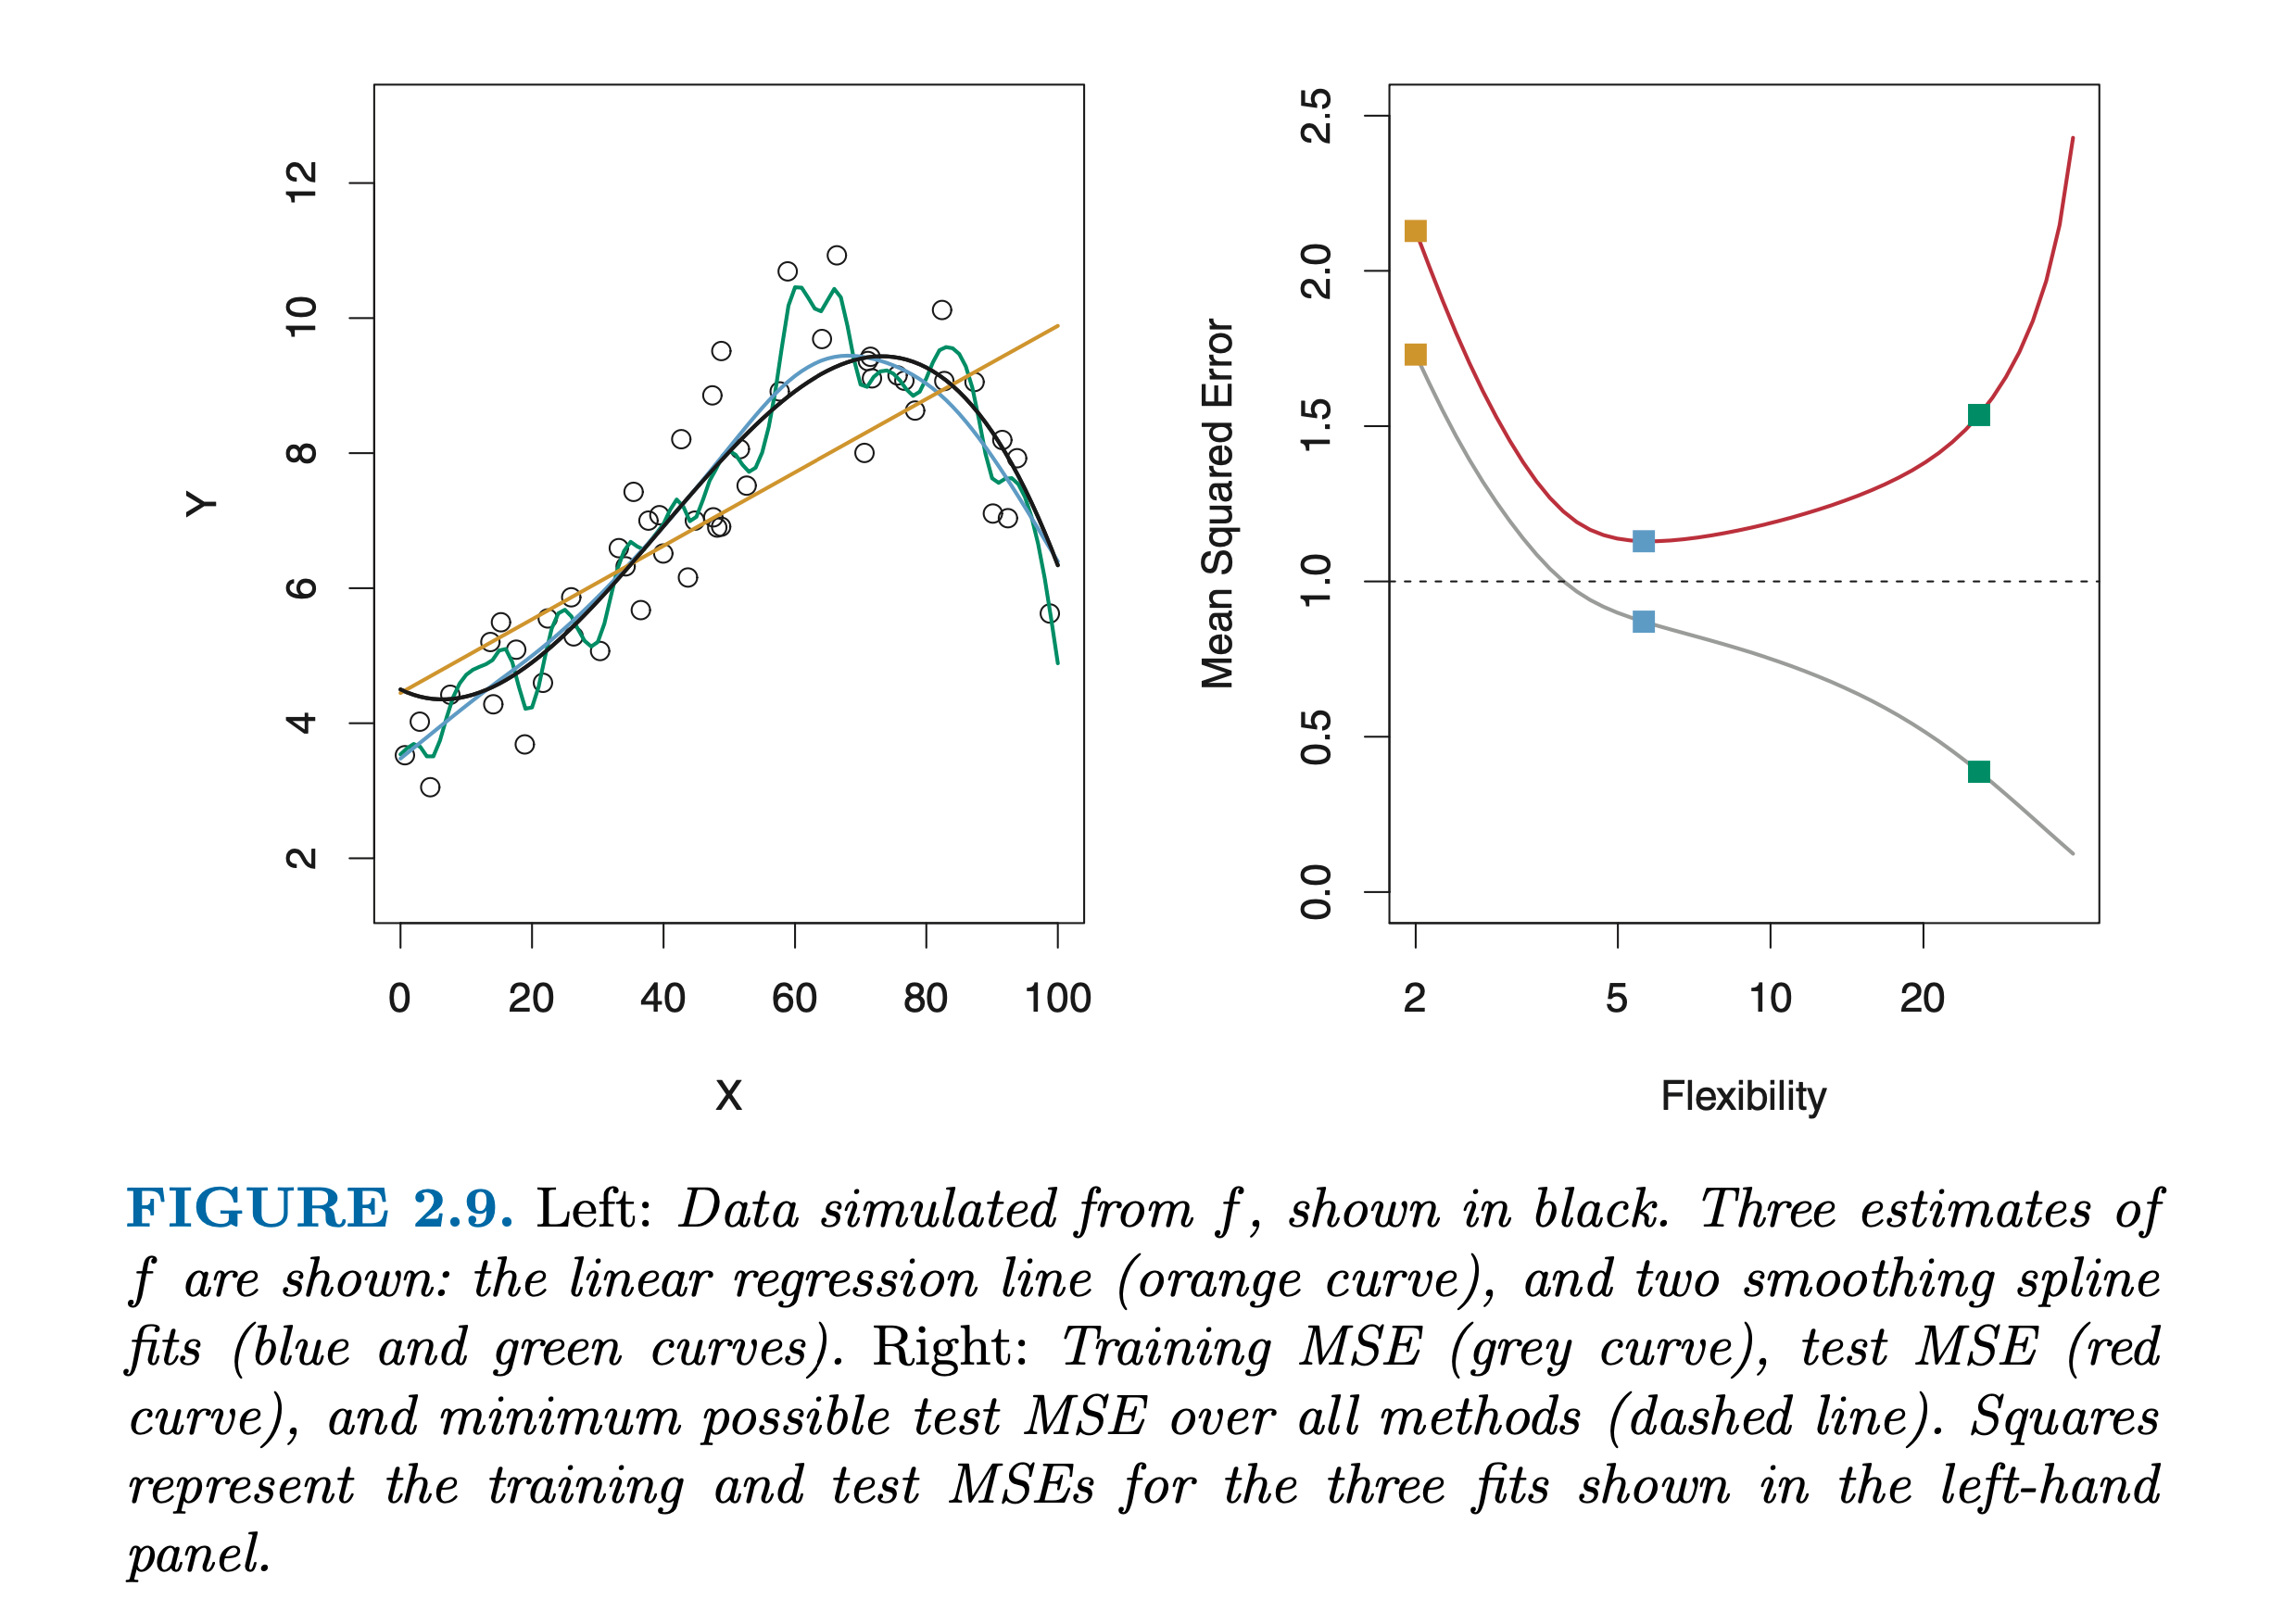
\includegraphics{fig2.9.png}

As the flexibility of the statistical learning method increases, we
observe a monotone decrease in the training MSE and a \(U\)-\emph{shape}
in the test MSE. This is a fundamental property of statistical learning
that holds regardless of the particular data set at hand and regardless
of the statistical method being used. AS model flexibility increases,
training MSE will decrease, but the test MSE may not. When a given
method yields a small training MSE but a large test MSE, we are said to
be \emph{overfitting} the data. This happens because our statistical
learninig procedure is working too hard to find patterns in the training
data, and may be picking up some patterns that are just caused by random
change rather than by true properties of the unknown function \(f\).
When we overfit the trainin data, the test MSE will be very large
because the supposed patterns that the method found in the training data
simply don't exist in the test data.

Note that regardless of whether or not overfitting has occured, we
almost always expect the training MSE to be smaller than the test MSE
because most statistical learning methods either directly or inderectly
seek to mimizie the training MSE. Overfitting refers specifically to the
case in which a less flexible model would have yielded a smaller test
MSE.

In practice, training MSE is computed easily, but estimating test MSE is
hard because usually no test data are available. We will learn
approaches that can be used in practice to estimate the mininmum test
MSE. One important method is \emph{cross-validation}( Chapter 5), which
is a method for estimating test MSE using the training data.

\hypertarget{the-bias-variance-trade-off}{%
\subsection{The Bias-Variance
Trade-Off}\label{the-bias-variance-trade-off}}

The U-shape in the test MSE result of two competing properties of
statistical learnig methods. The expected test MSE, for a given value
\(x_0\) can always be decomposed into sum of \emph{variance} of
\(\hat{f}(x_0)\), the squared \emph{bias} of \(\hat{f}(x_0)\) and the
variance of the error terms \(\epsilon\). That is

This means that to minimize the expected test error, we need to
simultaneously have \emph{low variance} and \emph{low bias}. Since
variance is always bigger than zero; \(\text{Var}(\epsilon)\), and
\(\text{Bias}(\hat{f}(x_0))\) are nonnegative. So, the expected test MSE
can never lie below \(\text{Var}(\epsilon)\), the irreducible error from
(2.3).

What do we mean by the \emph{variance} and \emph{bias} of statistical
learning method?

\emph{Varince} refers to the amount by which \(\hat{f}\) would change if
we estimated it using a different training data set; different training
data sets will result in a different \(\hat{f}\). But ideally,
\(\hat{f}\) should not vary too much between training sets. If a method
has high variance small changes in the training data can result in large
changes in \(\hat{f}\).

Flexible methods have hiher variance, because they fit better to the
data points and changing any of the data points may cause the estiamte
\(\hat{f}\) to chance considerably. But for example, least squares
method is relatively inflexible and has low variance, because mooving
any single observation will cause only a small shift in the position of
the line.(2.9)

\emph{bias} refers to the error that is due to functional form of
\(\hat{f}\). In real life, linear relationships are very rare. So
performing linear regression will result in some bias in the estimate of
\(f\). If your \(f\) is non-linear performing linear regression on
different data sets will not produce an accurate estimate; so linear
regression will result in high bias.

For example in 2.9 true \(f\) is non linear; so linear regression have
high bias, low variance. 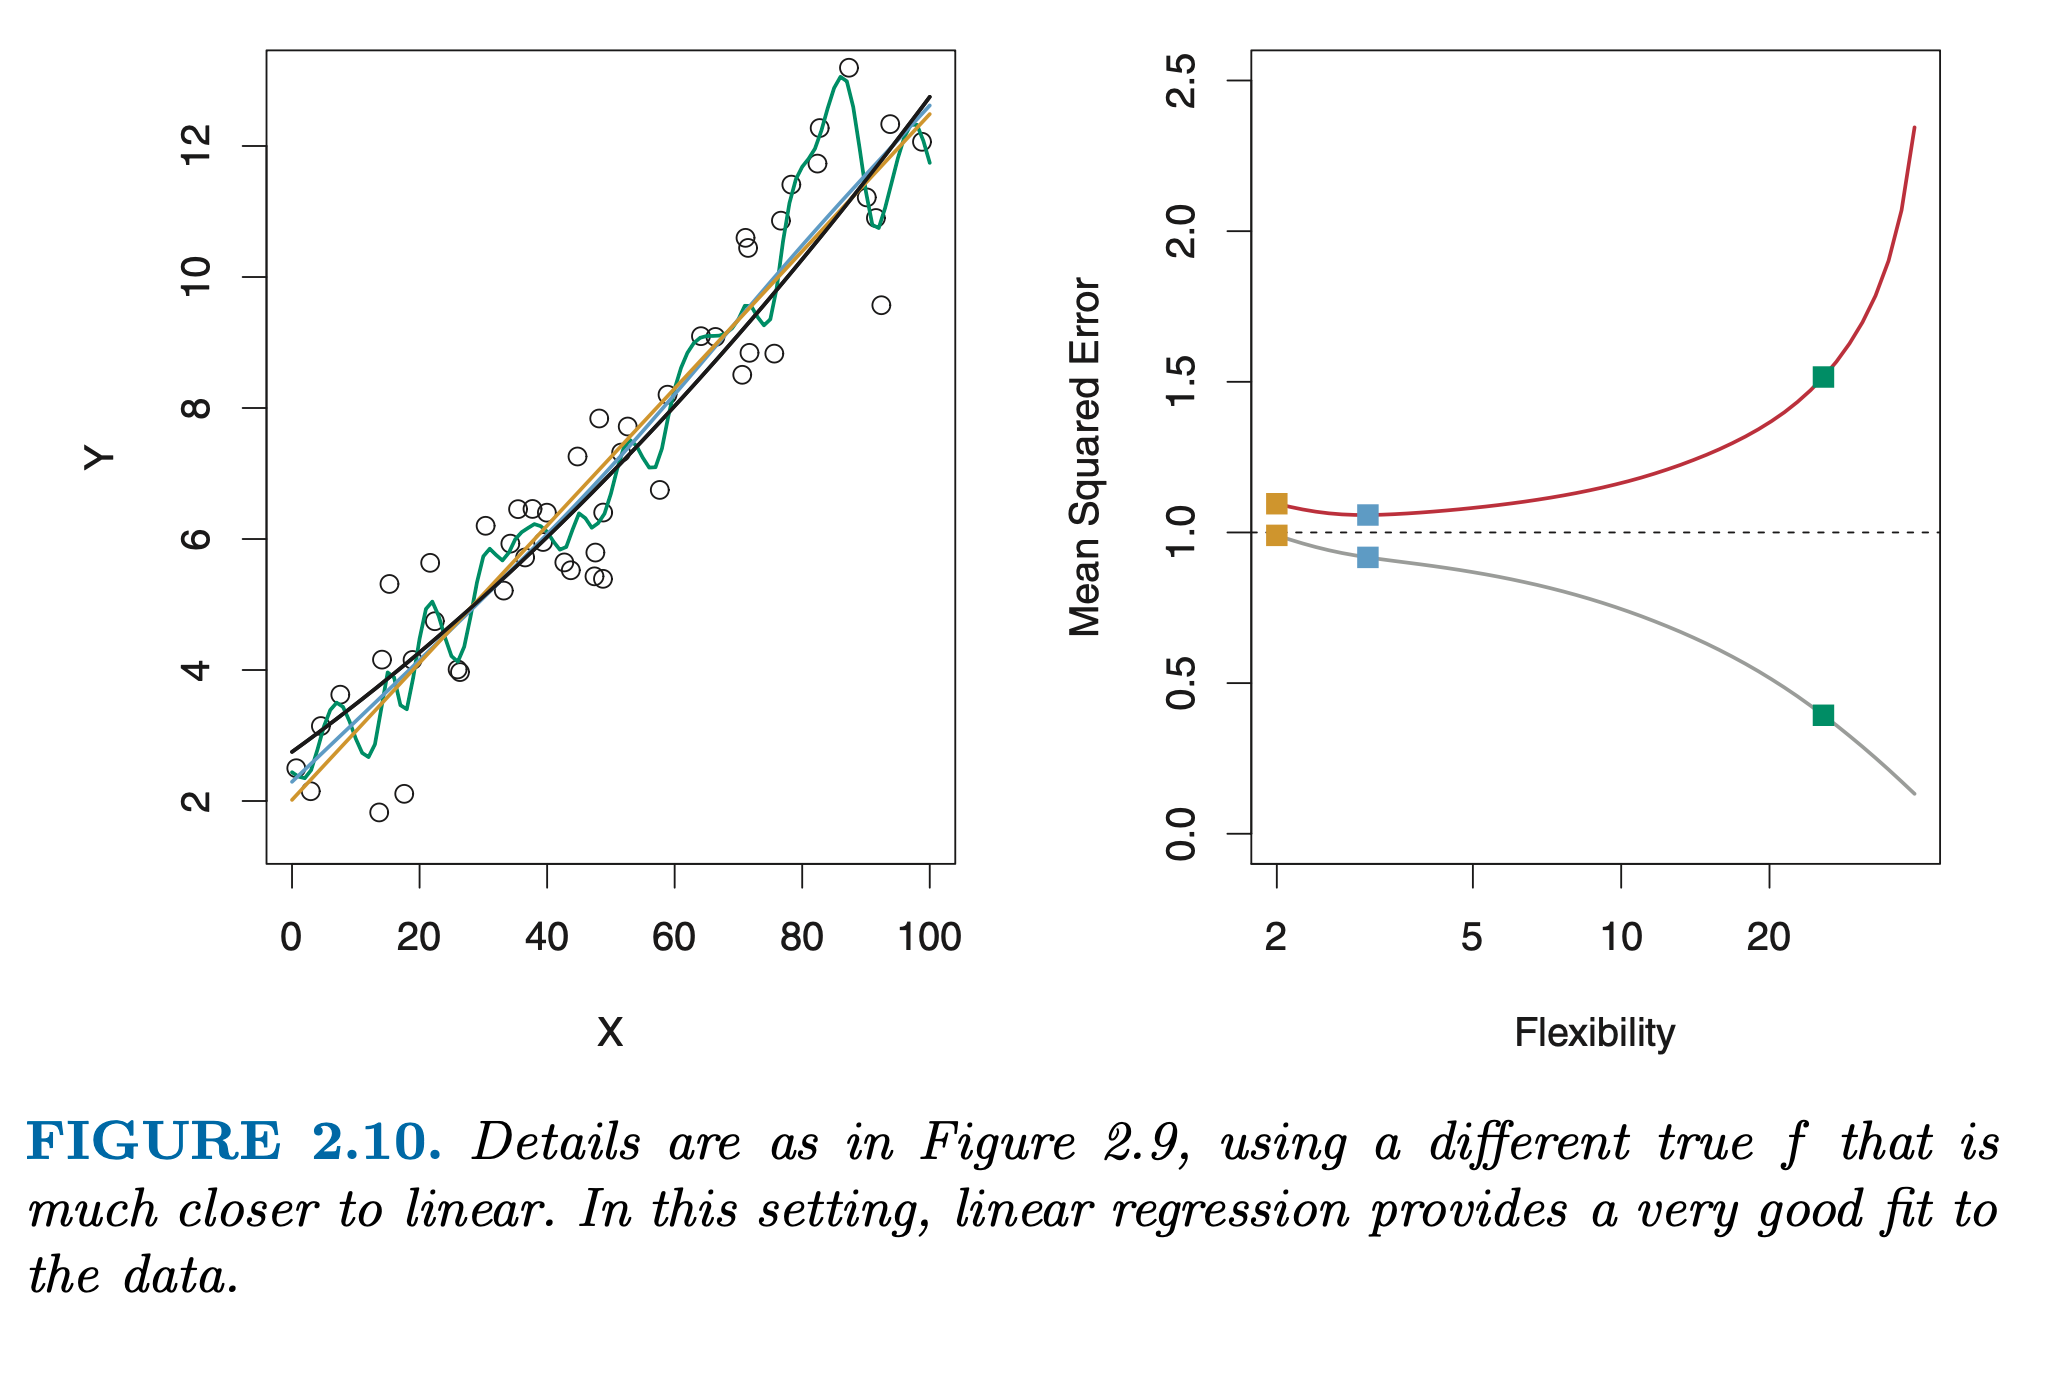
\includegraphics{fig2.10.png}

In 2.10 true \(f\) is very close to linear, so linaer regression have
low bias, low variance.

Generally more flexible methods result in less bias.

As a general rule, as we use more flexible methods the variance will
increase and bias will decrease. The relative rate of change of these
two quantities determines whether test MSE increases or decreases. As we
increase the flexibility, the bias tends to initially decrease faster
than the variance increases =\textgreater{} test MSE declines. However,
at some point increasing flexibility has little impact on thebias but
starts to significantly increase the variance =\textgreater{} test MSE
increases.

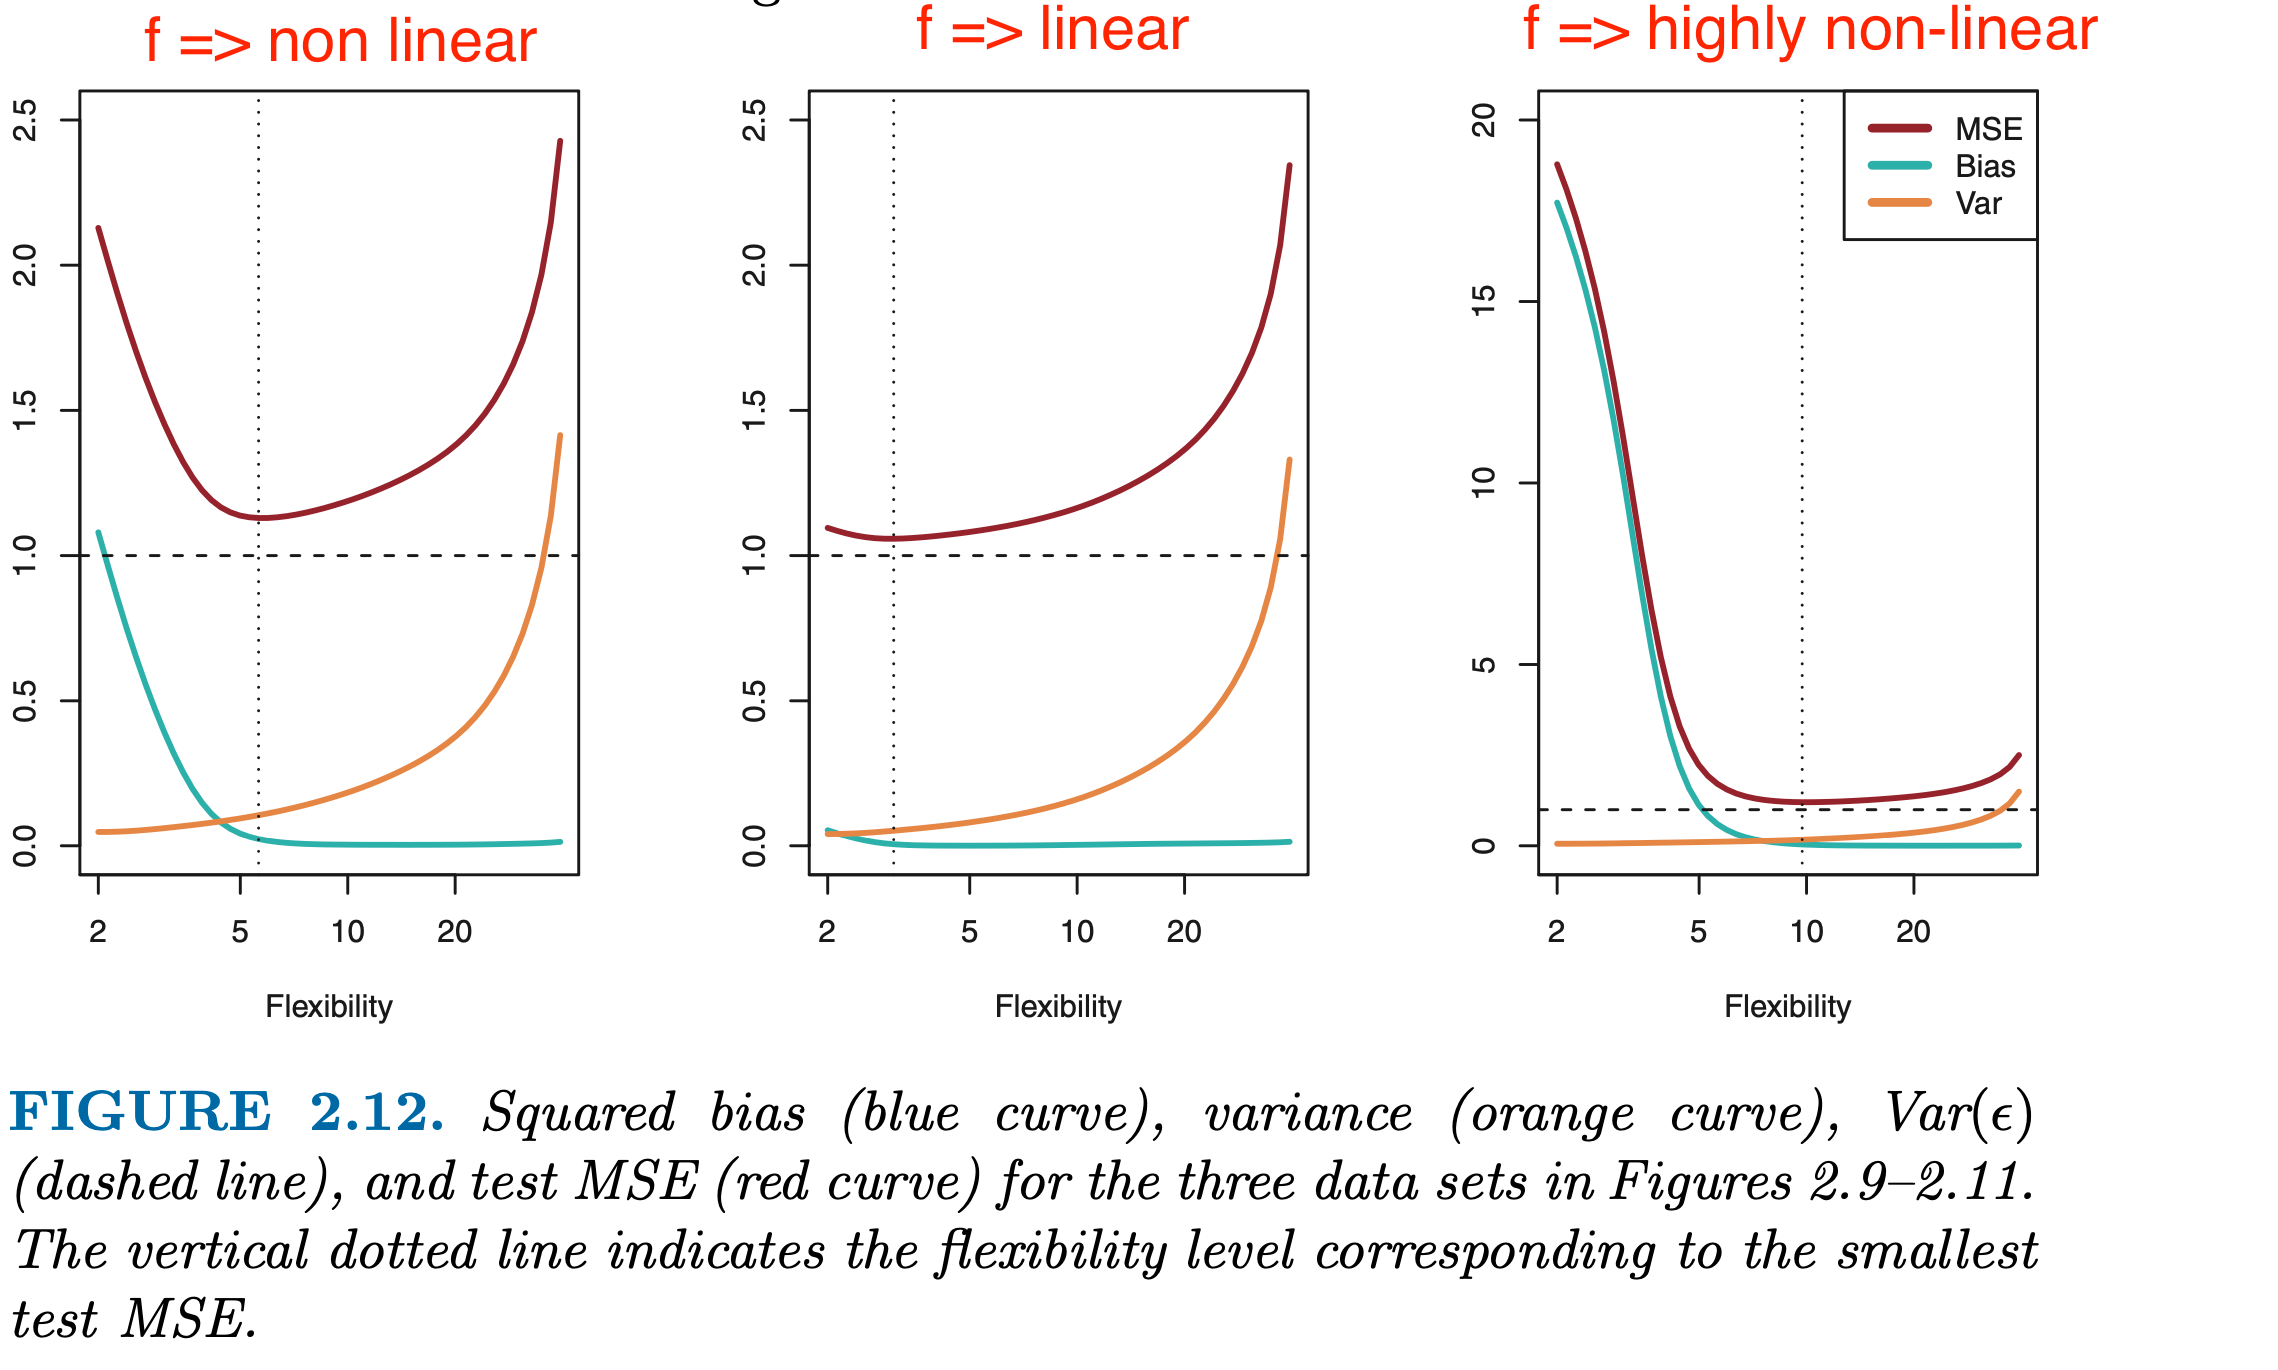
\includegraphics{fig2.12.png}

Figure 2.12 shows bias and variance effect to the test MSE for different
\(f\)s. Horizontal dashed line represents \(\text{Var}(\epsilon)\), the
irreducible error; the red curve test MSE is the sum of squared bias,
variance, and variance of irreducible error. In all cases bias decreases
as flexibility increaes. However, the optimal flexibility is different
for each \(f\). In the left panel the bias initially decreaes rapidly,
decreasing test MSE. In center panel true \(f\) is closer to linear so
there is only a small decrease in bias as flexibility increaes, and the
test MSE only declines slightly before increasing rapidly as the
variance increaes. Right hand panel, as flexibility increaess bias
dramatically decreases because true \(f\) is very non-linear. There is
alsso very little increase in variance as flexibility increases
=\textgreater{} tets MSE decreases before increasing.

This is called bias-variance trade off. Good test set performance of a
method requires low variance as well as low squared bias. This is a
trade off because it is easy to obtain a method with extremely low bias
but high variance(for instance, drawing a curve that passes through
every single training observation, or a method with low variance but
high bias(by fitting a horizontal line to the data). Challange is
finding a method wihch both the variance and squareed bias are low.

In real life, it is not possible to explicitly compute the test MSE,
bias, or variance for methods. But we should keep this in mind.

\hypertarget{the-classification-setting}{%
\subsection{The Classification
Setting}\label{the-classification-setting}}

So far we focused on regression setting. Problems such as bias-variance
trade of also occurs in classification but in a modificated way because
\(y_i\) is no longer numerical.

Suppose that we seek to estiamte \(f\) on the basis of training
observations \(\{(x_1,y_1), \dots, (x_n,y_n)\}\) where now
\(y_1,\dots, y_n\) are qualitative.

We need to quantify the accuracy of our estimate \(\hat{f}\). We can use
the training \emph{error rate}, the proportion of mistakes that are made
if we apply our estimate \(\hat{f}\) to the training observations:

\[
\text{error rate}=\frac{1}{n}\sum^n_{i=1}I(y_i \neq \hat{y_i})
\] (2.8)

\(\hat{y_i}\) is the predicted class label for the \(i\)th observation
using \(\hat{f}\). \(I(y_i \neq \hat{y_i})\) is an \emph{indicator
variable} that equals 1 if \(y_i \neq \hat{y_i}\) and zero if
\({y_i = \hat{y_i}}\). If \(I(y_i \neq \hat{y_i}) = 0\) then \(i\)th
observation was classified correctly, otherwise it was misclassified. So
(2.8) computes the fraction of incorrect classifications.

(2.8) is \emph{training error}. But as the regression setting we are
more interested in \emph{test error} rate. The \emph{test error} rate
associated with a set of test observations of the form

\[
\text{error rate}_{test} = \frac{1}{n_{test}}\sum_{i=1}^{n_{test}}(I(y_{test_i} \neq \hat{y}_{test_i}))
\] (2.9)

A \emph{good} classifier is one for which the test error is smallest.

\textbf{The Bayes Classifier}

We can minimize test error rate by a very simple classifier that
\emph{assigns each observation to the most likely class, given its
predictor values}. In other words, we should simply assign a test
observation with predictor vector \(x_0\) to the class \(j\) for which

\[
Pr(Y = j | X = x_0)
\] (2.10)

is largest. This is \emph{conditional probability:} it is the probabilty
that \(Y=j\) given the observed predictor vector \(x_0\). This
classifier is called \emph{Bayes classifier}.

In a two-class problem where there are only two possible response
values, \emph{class 1} or \emph{class2}, the Bayes classifier
corresponds to predicting class one if \(Pr(Y=1 | X = x_0) > 0.5\), and
class two otherwise.

Imagine having \(X = (X_1, X_2)\). For each value of \(X_1\) and \(X_2\)
there will be a different probability of the response being class 1 or
2. For \(Pr(Y=class1 | X = (X_2,X_2)) > 0.5\) and
\(Pr(Y=class2 | X = (X_1,X_2))\).

The Bayes classifier produces the lowest possible test error rate,
called the \emph{Bayes error rate}. Since the Bayes classifer will
always choose the class for which \(Pr(Y = j | X = x_0)\) is largest,
the error rate at \(X=x_0\) will be \(1-\max_jPr(Y =j | X = x_0)\). In
general, the overall Bayes error rate is given by

\[
\text{Bayes error rate} = 1 - E(\max_jPr(Y =j | X))
\] (2.11)

where the expectation averages the probabilty over all possible values
of X. The Bayes eror rate is analogous to the irreducible eror.

\textbf{K-Nearest Neighbors}

In theory we always want to predict qualitative responses using the
Bayes classifier. But for real data, we do not know the conditional
distribution of \(Y\) given \(X\), and so computing the Bayes classfier
is impossible. So Bayes classifier is like a gold standard to compare
other methods.

Many approaches attemp to estiamte the conditional distribution of \(Y\)
given \(X\), and then classify a given observation to the class with
highest \emph{estimated} probability. One of them is \emph{K-nearest
neighbors}(KNN) classfier.

Given a positive integer \emph{K} and a test observation \(x_0\), the
KNN clasffier first identifies the \emph{K} points in the training data
that are closest to \(x_0\), represented by \(N_0\). It then esitmates
the conditional probability for class \emph{j} as the fraction points in
\(N_0\) whose response values equal to \(j\).

\[
Pr(Y = j | X = x_0) = \frac{1}{K}\sum_{i \in N_0}I(y_i=j)
\] (2.12)

Finally, KNN applies Bayes rule and classifies the test observation
\(x_0\) to the class with the largest probability.

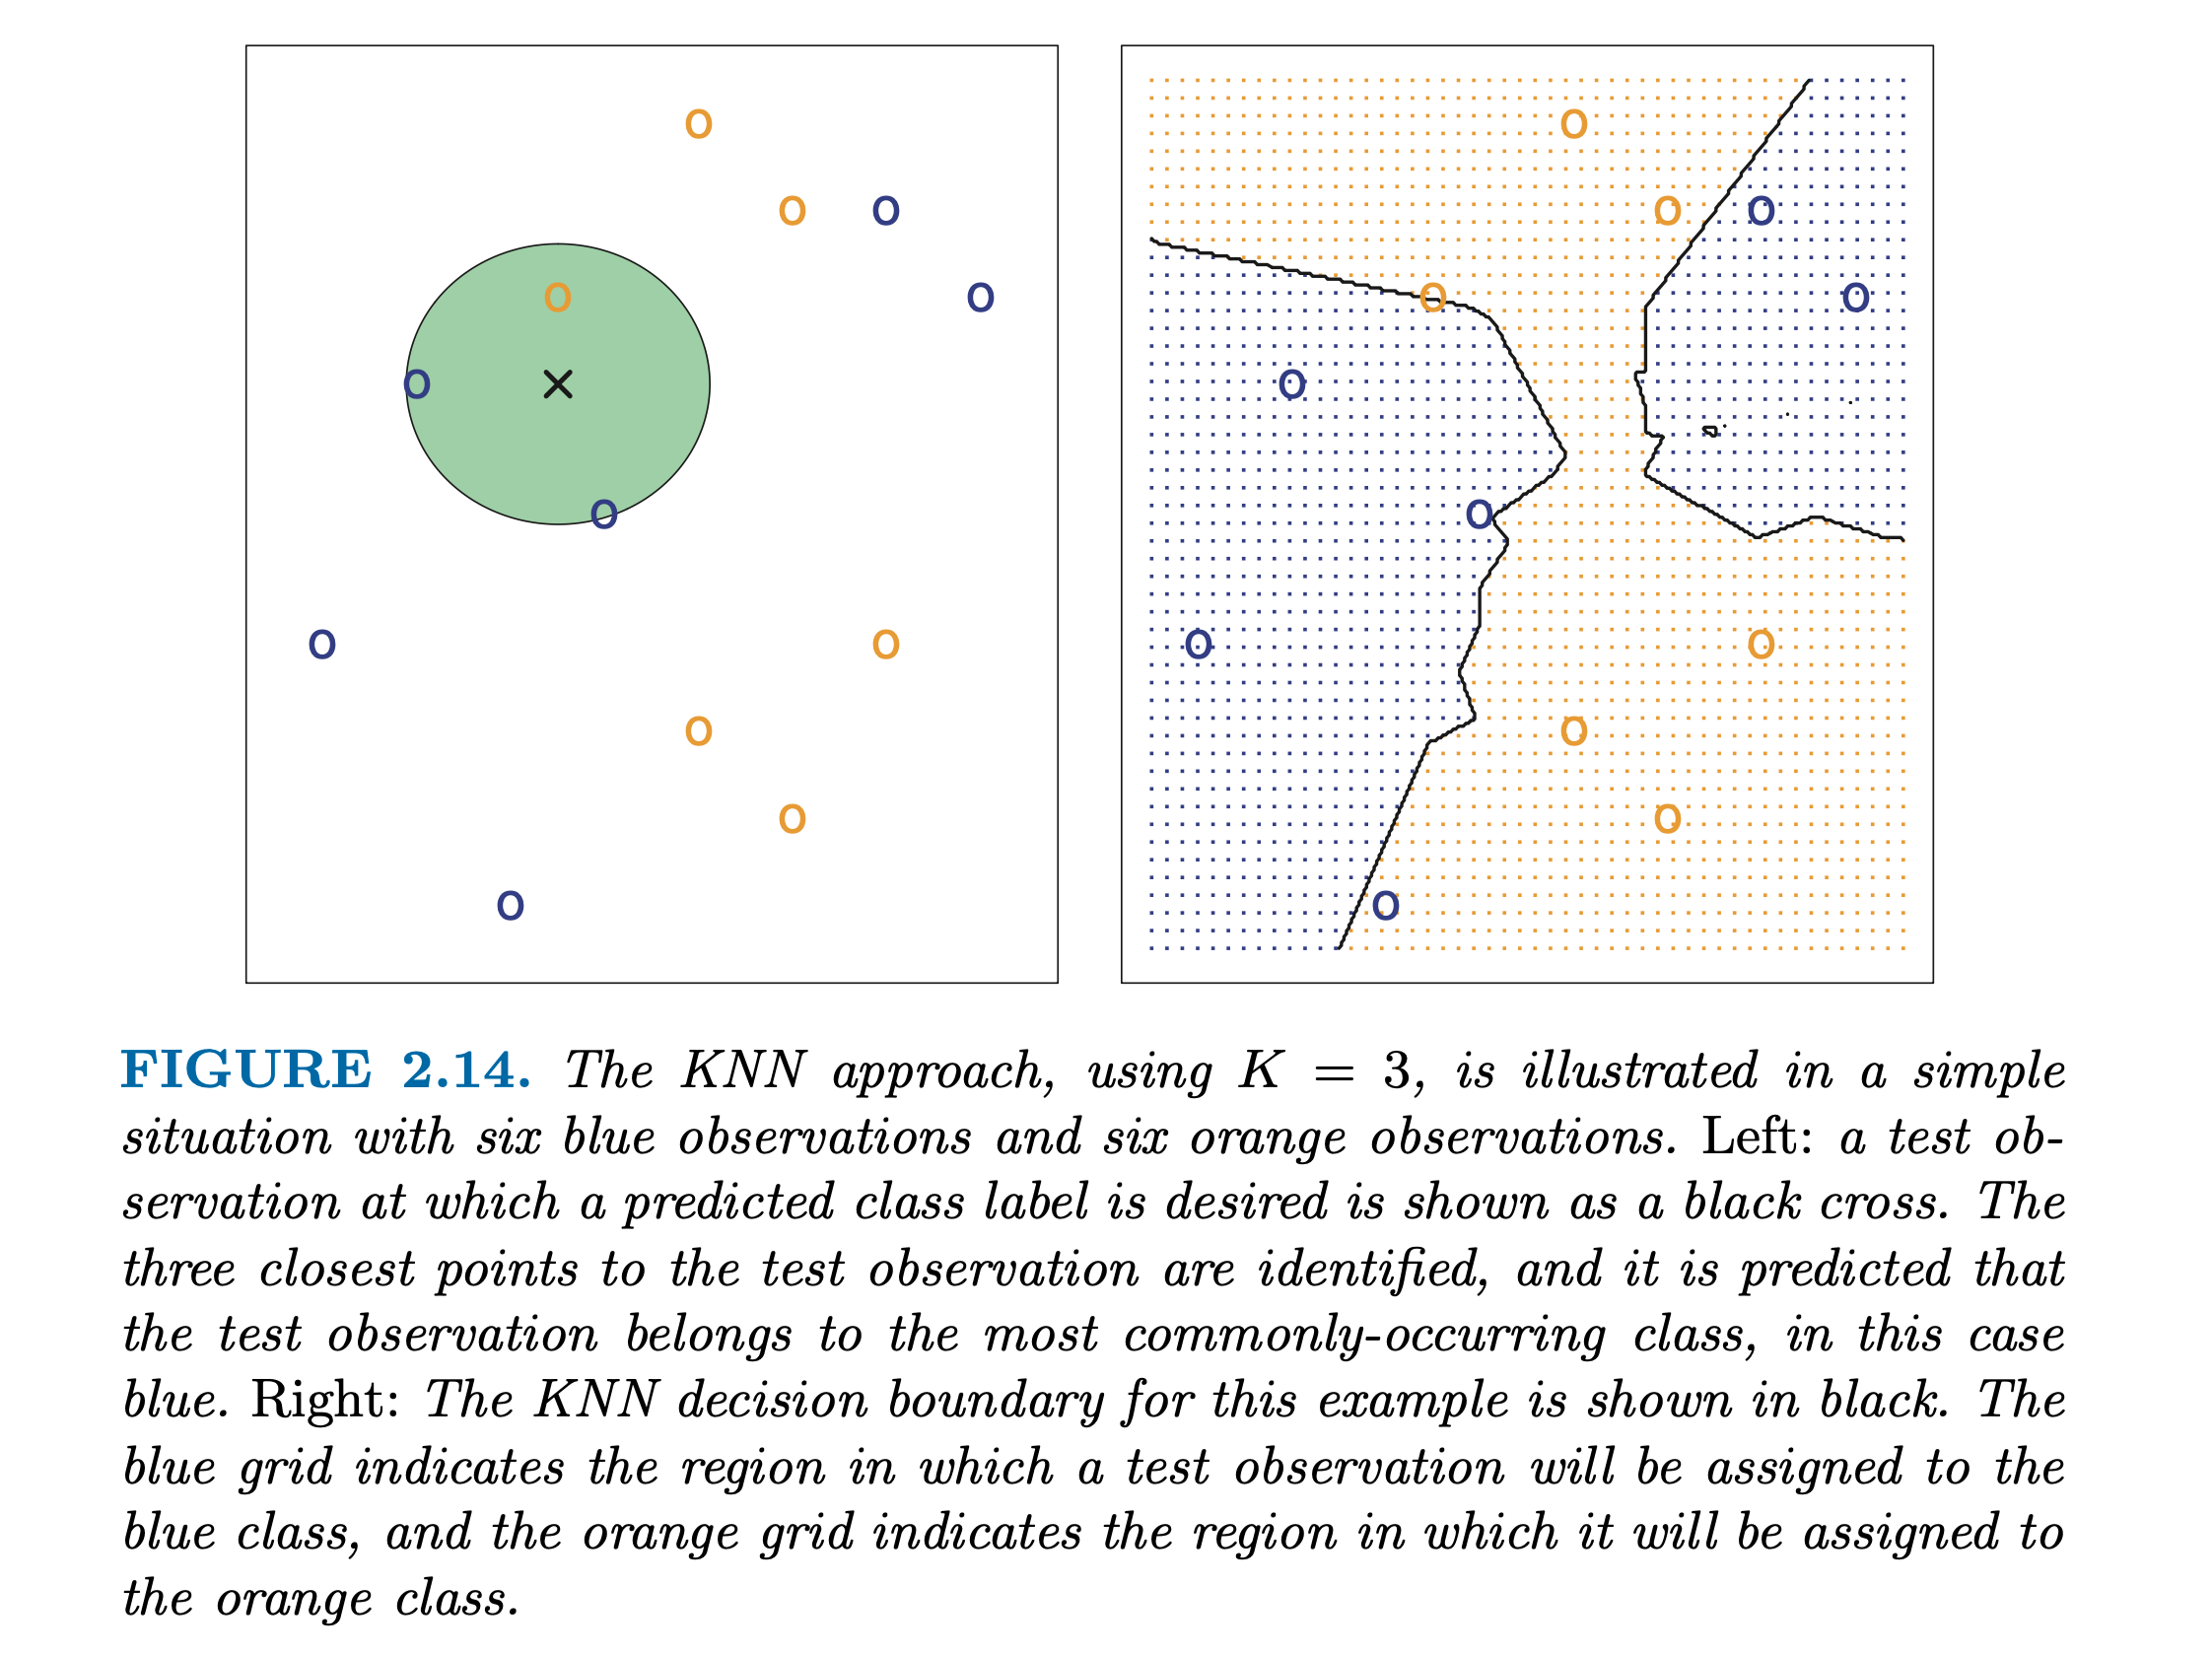
\includegraphics{fig2.14.png}

Figure 2.14 provides an illustrative example of the KNN approach. Left
panel =\textgreater{} Our goal is to make prediction for the black cross
point. When \(K=3\) KNN will identify the 3 oservations that are closest
to the cross. There are two blue and one orange points;
\(Pr(Y=orange | X = x_{cross}) = 1/3\), and
\(Pr(Y=blue | X = x_{cross}) = 2/3\) =\textgreater{} KNN will predict
that the black cross belongs to the blue class.

The choice of K is very important. as K increases flexibility decreases
=\textgreater{} high bias, but low variance.

Just like in regression setting there is not a strong relationship
between the training error rate and the test error rate.

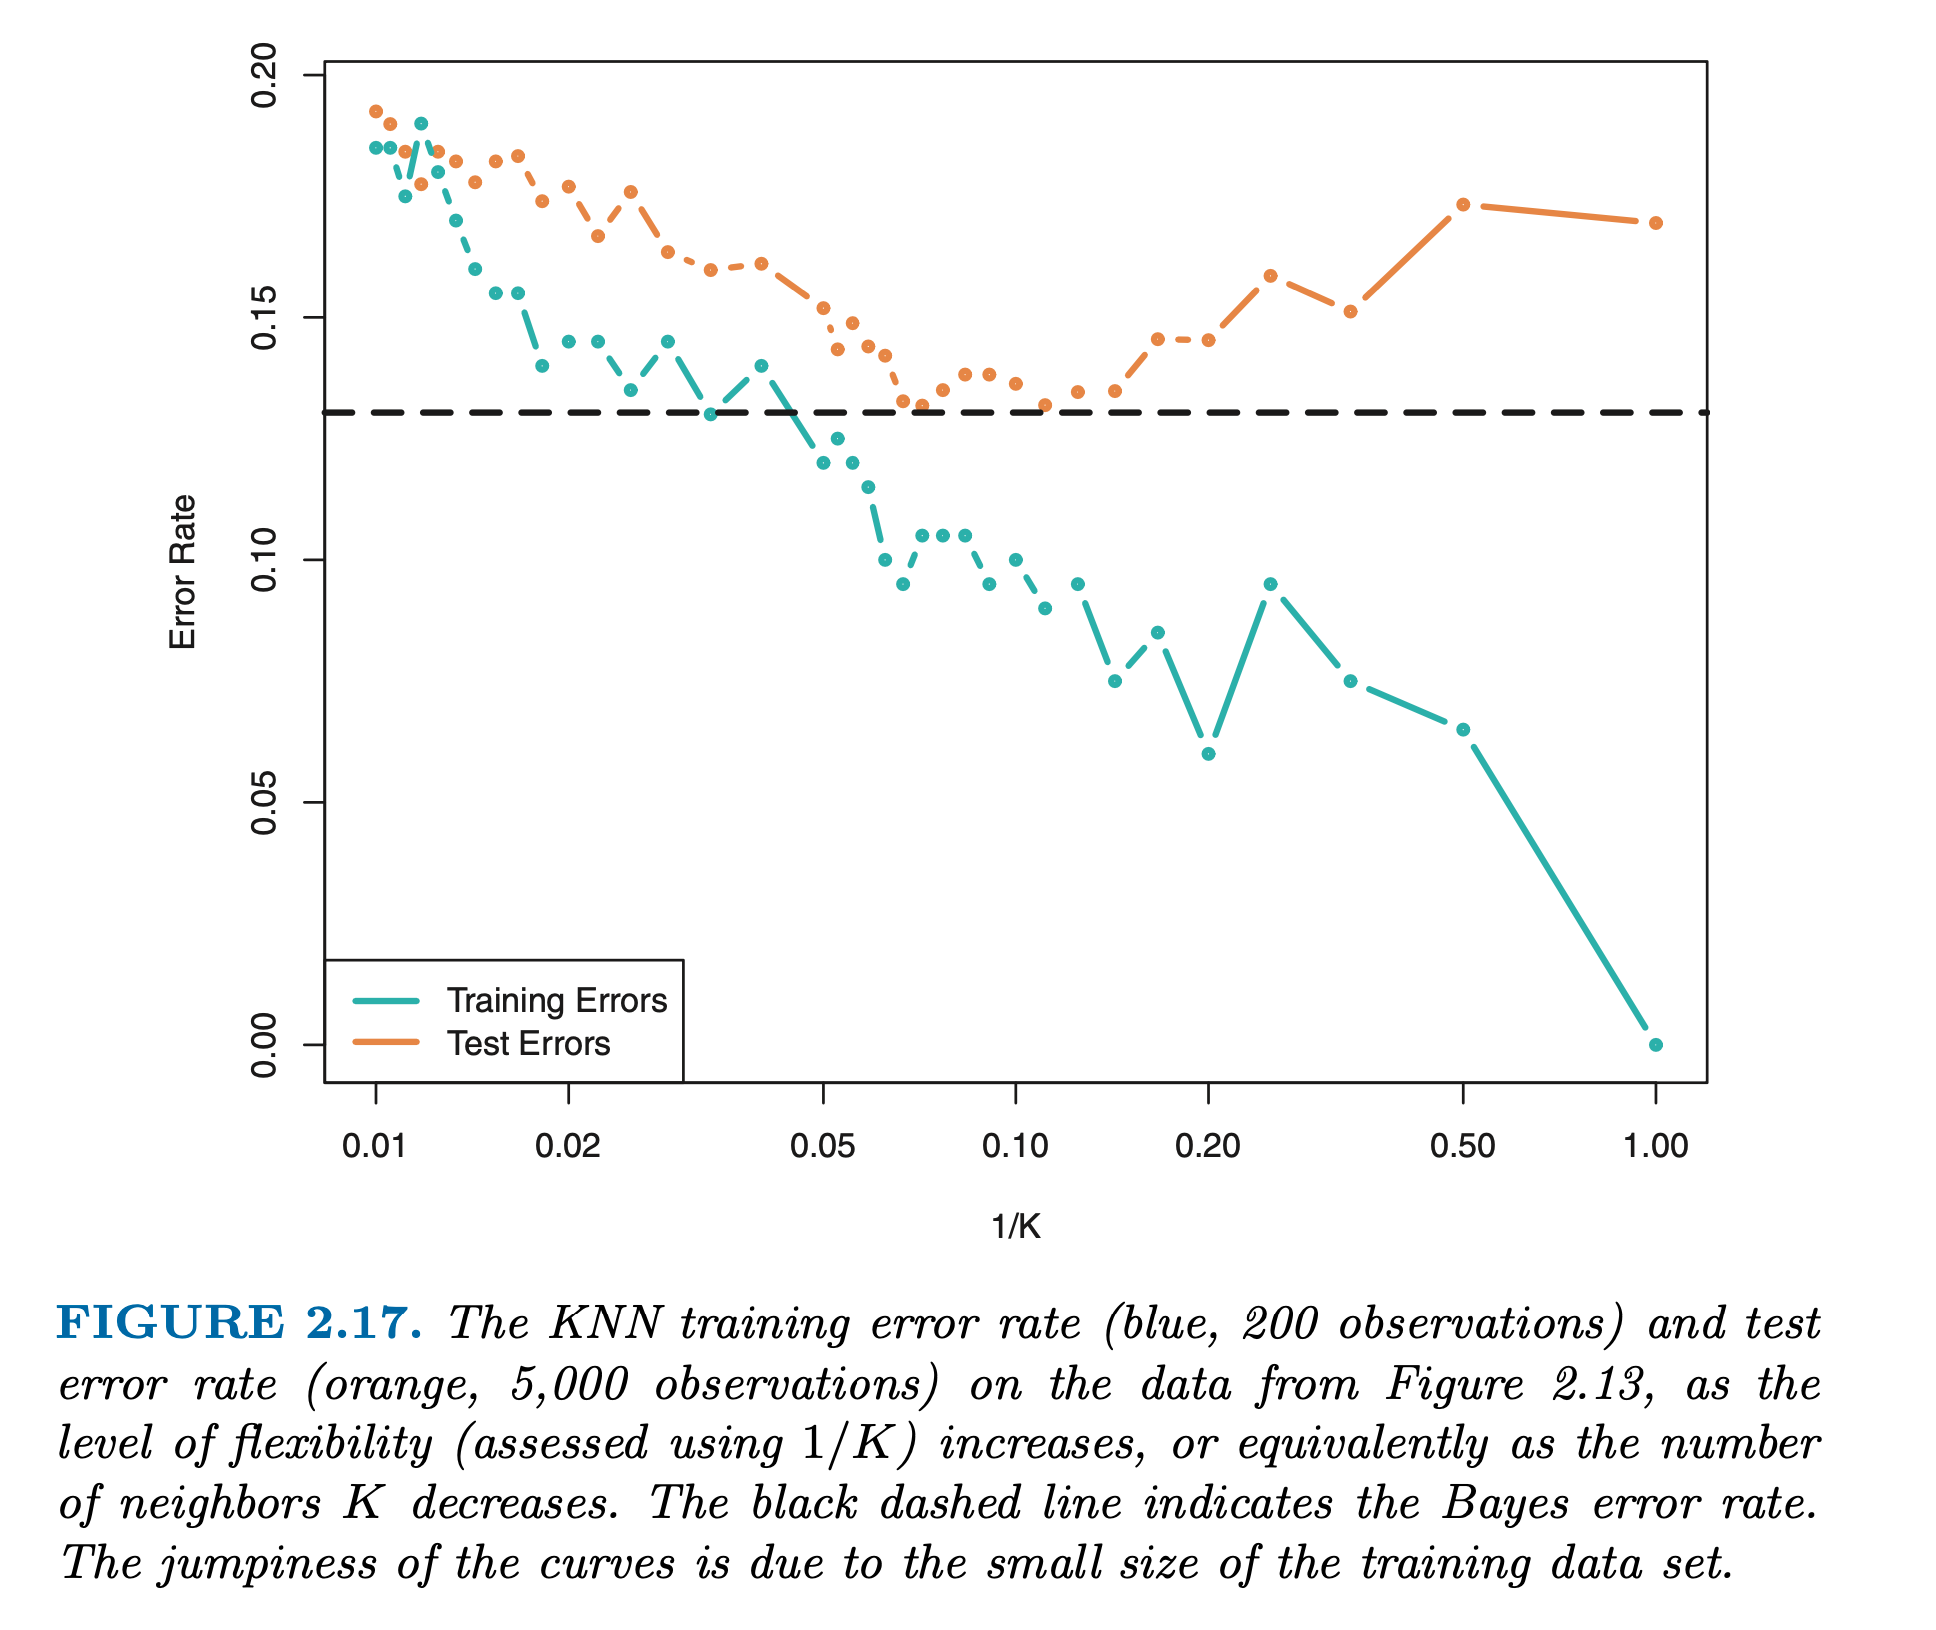
\includegraphics{fig2.17.png}

as in the regression setting, the training error rate consistently
declines as the flexibility(\(1/K\)) increases. However, the test error
rate again have a characteristic U-shape.

In both regression and classification settings, choosing the correct
level of flexibility is critical. The bias-variance tradeoff
=\textgreater{} U-shape in the test error, can make this a difficult
task.

\bookmarksetup{startatroot}

\hypertarget{linear-regression}{%
\chapter{Linear Regression}\label{linear-regression}}

We will predict quantitative response.

\begin{Shaded}
\begin{Highlighting}[]
\NormalTok{advertising }\OtherTok{=} \FunctionTok{read\_csv}\NormalTok{(}\StringTok{"./data/Advertising.csv"}\NormalTok{) }\SpecialCharTok{\%\textgreater{}\%}\NormalTok{ as\_tibble }\SpecialCharTok{\%\textgreater{}\%} \FunctionTok{select}\NormalTok{(}\SpecialCharTok{{-}}\DecValTok{1}\NormalTok{)}
\NormalTok{advertising}
\end{Highlighting}
\end{Shaded}

\begin{verbatim}
# A tibble: 200 x 4
      TV radio newspaper sales
   <dbl> <dbl>     <dbl> <dbl>
 1 230.   37.8      69.2  22.1
 2  44.5  39.3      45.1  10.4
 3  17.2  45.9      69.3   9.3
 4 152.   41.3      58.5  18.5
 5 181.   10.8      58.4  12.9
 6   8.7  48.9      75     7.2
 7  57.5  32.8      23.5  11.8
 8 120.   19.6      11.6  13.2
 9   8.6   2.1       1     4.8
10 200.    2.6      21.2  10.6
# i 190 more rows
\end{verbatim}

We are asked to suggest a marketing plan for next year which will yeild
high product sales. We may want to inquire the following questions:

\begin{enumerate}
\def\labelenumi{\arabic{enumi}.}
\item
  \emph{Is there a relationship between advertising budget and sales?}

  First we should determine if there is an association between
  adveritisng expenditure and sales. If not, no money shpuld be spent on
  advertising.
\item
  \emph{How strong is the relationship between advertising budget and
  sales?}

  If there is a relationship between advertising and sales, what is the
  strength of this relationship? Given a certain advertising budget, can
  we predict sales with a high level of accuracy? =\textgreater{} strong
  relationsihp.
\item
  \emph{Which media contribute to sales?}

  Do all variables--tv,radio,newspaper-- contribute to sales, or just
  one or the two?
\item
  \emph{How accurately can we estimate the effect of each medium on
  sales?}

  For every ollar spent on advertising in a particular medium, by what
  amount will sales increase? How accuretly can we predict this amount
  of increase?
\item
  \emph{How accurately can we predict future sales?}

  For any given level of media advertisig, what is our prediction for
  sales, and what is the accuracy of this prediciton?
\item
  \emph{Is the relationship linear?}

  If so linear regresion is appropriate tool, if not we may need to
  transform the predictor or the repsonse so that liner regression can
  be used.
\item
  \emph{Is there synergy among the advertising media?}

  Does the effect of a medium on sales depend on other medium levels?
  Does dividing advertisement budget to two or three medium yeild a
  higher sales?
\end{enumerate}

We can answer each of these questions using Linear regression.

\hypertarget{simple-linear-regression}{%
\section{Simple Linear Regression}\label{simple-linear-regression}}

Predicting a quantitative response \(Y\) on the basis of a single
predictor variable \(X\).

Our assumption is that there is approximately a linear relationship
between \(X\) and \(Y\); we can write this linear relationship as

\[
Y = \beta_0 + \beta_1 X_1 + \epsilon
\]

\[
Y \approx \beta_0 + \beta_1X
\] (3.1)

For example lets say \(X\) is \texttt{TV}, and \(Y\) is \texttt{sales}

\[
sales = \beta_0 + \beta_1 \times TV + \epsilon
\] or

\[
sales = \beta_0 + \beta_1 \times TV
\]

On (3.1) \(\beta_0\) and \(\beta_1\) are unknown constants that
represent the \emph{intercept} and \emph{slope} in the linear model.
Together they are known as \emph{coefficients} or \emph{parameters}.

We are going to use or training data to produce estimates for
\(\beta_0\) =\textgreater{} \(\hat{\beta_0}\) and \(\beta_1\)
=\textgreater{} \(\hat{\beta_1}\). Using these predicted coefficients we
can predict sales;

\[
\hat{sales} = \hat{\beta_0} + \hat{\beta_1} \times TV
\]

or as in general form

\[
\hat{y} = \hat{\beta_0} + \hat{\beta_1}x
\] (3.2)

\hypertarget{estimating-the-coefficients}{%
\subsection{Estimating the
coefficients}\label{estimating-the-coefficients}}

Since, \(\beta_0\) and \(\beta_1\) are unknown, before we can use (3.1)
to make predictions we must use data to estimate the coefficients. We
have \(n\) observations :

\[
(x_1,y_1), (x_2,y_2), \dots, (x_n,y_n)
\]

We want our estimated coefficients to give such predictions that will
fit the avaible data as well =\textgreater{}
\(y_i \approx \hat{\beta_0} + \hat{\beta_1}x_i\) for \(i = 1,\dots, n\).
This coefficients will allow us to draw a regression line and we want
this regression line to be close as possible to the \(n\) data points we
have.

There are different ways to measure \emph{closeness}. The most common
approach is minimizing the \emph{least squares} criterion. Alternative
approaches will be considered in Chapter 6.

Our predictions come from
\(\hat{y_i} = \hat{\beta_0} + \hat{\beta_1}x_i\).

Then for each data we have a \emph{residual}: difference between \(y\)
and \(\hat{y}\):

\[
e_i = y_i - \hat{y_i}
\]

We need to take the squares to get the distances--because of the
negative residuals, and sum them to get the \emph{residual sum of
squares}(RSS)

\[
RSS = e_1^2 + e_2^2 + \dots + e_n^2
\]

this is equal to

\[
RSS = (y_i - \hat{beta_0} - \hat{\beta_1}x_1)^2 + (y_2 - \hat{\beta_0} - \hat{\beta_1}x_2) + \dots + (y_n - \hat{\beta_0} - \hat{\beta_1}x_n)
\] (3.3)

The least squares approach chooses \(\hat{\beta_0}\) and
\(\hat{\beta_1}\) to minimize RSS. These minimizers are

\[
\begin{align}
\hat{\beta_1} &= \frac{\sum_{i=1}^n(x_i - \bar{x})(y_i - \bar{y})}{\sum_{i=1}^n(x_i - \bar{x})^2} \\
\hat{\beta_0} &= \bar{y_i} - \hat{\beta_1}\bar{x}
\end{align}
\] (3.4)

\(\bar{y} = \frac{1}{n}\sum_{i=1}^ny_i\) and
\(\bar{x} = \frac{1}{n}\sum_{i=1}^nx_i\) are the sample means.

So (3.4) defines the \emph{least squares coefficient estimates} for
simple linear regression.

Lets calculate them with R

\begin{Shaded}
\begin{Highlighting}[]
\NormalTok{beta\_1\_hat\_adv }\OtherTok{=} \FunctionTok{sum}\NormalTok{((advertising}\SpecialCharTok{$}\NormalTok{TV }\SpecialCharTok{{-}} \FunctionTok{mean}\NormalTok{(advertising}\SpecialCharTok{$}\NormalTok{TV)) }\SpecialCharTok{*}\NormalTok{ ((advertising}\SpecialCharTok{$}\NormalTok{sales }\SpecialCharTok{{-}} \FunctionTok{mean}\NormalTok{(advertising}\SpecialCharTok{$}\NormalTok{sales)))) }\SpecialCharTok{/} \FunctionTok{sum}\NormalTok{((advertising}\SpecialCharTok{$}\NormalTok{TV }\SpecialCharTok{{-}} \FunctionTok{mean}\NormalTok{(advertising}\SpecialCharTok{$}\NormalTok{TV))}\SpecialCharTok{\^{}}\DecValTok{2}\NormalTok{)}
\NormalTok{beta\_1\_hat\_adv}
\end{Highlighting}
\end{Shaded}

\begin{verbatim}
[1] 0.04753664
\end{verbatim}

So; our \$\hat{\beta_1} = 0.0475 \$

\begin{Shaded}
\begin{Highlighting}[]
\NormalTok{beta\_0\_hat\_adv }\OtherTok{=} \FunctionTok{mean}\NormalTok{(advertising}\SpecialCharTok{$}\NormalTok{sales) }\SpecialCharTok{{-}}\NormalTok{ beta\_1\_hat\_adv }\SpecialCharTok{*} \FunctionTok{mean}\NormalTok{(advertising}\SpecialCharTok{$}\NormalTok{TV)}
\NormalTok{beta\_0\_hat\_adv}
\end{Highlighting}
\end{Shaded}

\begin{verbatim}
[1] 7.032594
\end{verbatim}

our \(\hat{\beta_0} = 7.032\)

Lets compare them with r function

\begin{Shaded}
\begin{Highlighting}[]
\FunctionTok{summary}\NormalTok{(}\FunctionTok{lm}\NormalTok{(sales }\SpecialCharTok{\textasciitilde{}}\NormalTok{ TV, }\AttributeTok{data =}\NormalTok{ advertising))}
\end{Highlighting}
\end{Shaded}

\begin{verbatim}

Call:
lm(formula = sales ~ TV, data = advertising)

Residuals:
    Min      1Q  Median      3Q     Max 
-8.3860 -1.9545 -0.1913  2.0671  7.2124 

Coefficients:
            Estimate Std. Error t value Pr(>|t|)    
(Intercept) 7.032594   0.457843   15.36   <2e-16 ***
TV          0.047537   0.002691   17.67   <2e-16 ***
---
Signif. codes:  0 '***' 0.001 '**' 0.01 '*' 0.05 '.' 0.1 ' ' 1

Residual standard error: 3.259 on 198 degrees of freedom
Multiple R-squared:  0.6119,    Adjusted R-squared:  0.6099 
F-statistic: 312.1 on 1 and 198 DF,  p-value: < 2.2e-16
\end{verbatim}

Calculating the predicted values

\begin{Shaded}
\begin{Highlighting}[]
\NormalTok{y\_hat\_adv }\OtherTok{=}\NormalTok{ beta\_0\_hat\_adv }\SpecialCharTok{+}\NormalTok{ beta\_1\_hat\_adv }\SpecialCharTok{*}\NormalTok{ advertising}\SpecialCharTok{$}\NormalTok{TV}
\NormalTok{y\_hat\_adv[}\DecValTok{1}\SpecialCharTok{:}\DecValTok{10}\NormalTok{]}
\end{Highlighting}
\end{Shaded}

\begin{verbatim}
 [1] 17.970775  9.147974  7.850224 14.234395 15.627218  7.446162  9.765950
 [8] 12.746498  7.441409 16.530414
\end{verbatim}

Our \(y_i\) values are as above.

\begin{Shaded}
\begin{Highlighting}[]
\NormalTok{RSS }\OtherTok{=} \FunctionTok{sum}\NormalTok{((advertising}\SpecialCharTok{$}\NormalTok{sales }\SpecialCharTok{{-}}\NormalTok{ y\_hat\_adv)}\SpecialCharTok{\^{}}\DecValTok{2}\NormalTok{)}
\NormalTok{RSS}
\end{Highlighting}
\end{Shaded}

\begin{verbatim}
[1] 2102.531
\end{verbatim}

Our \(\text{RSS} = 2102.531\)

So we can draw our regression line

\begin{Shaded}
\begin{Highlighting}[]
\NormalTok{advertising }\SpecialCharTok{\%\textgreater{}\%}
  \FunctionTok{ggplot}\NormalTok{() }\SpecialCharTok{+} \FunctionTok{aes}\NormalTok{(}\AttributeTok{x=}\NormalTok{TV, }\AttributeTok{y =}\NormalTok{ sales) }\SpecialCharTok{+}  \FunctionTok{geom\_abline}\NormalTok{(}\AttributeTok{intercept =}\NormalTok{ beta\_0\_hat\_adv, }\AttributeTok{slope =}\NormalTok{ beta\_1\_hat\_adv, }\AttributeTok{color =} \StringTok{"\#262B70"}\NormalTok{, }\AttributeTok{size =}\FloatTok{1.2}\NormalTok{) }\SpecialCharTok{+}
  \FunctionTok{geom\_segment}\NormalTok{(}\FunctionTok{aes}\NormalTok{(}\AttributeTok{xend=}\NormalTok{TV, }\AttributeTok{yend=}\NormalTok{y\_hat\_adv), }\AttributeTok{color =} \StringTok{"\#939393"}\NormalTok{) }\SpecialCharTok{+}
  \FunctionTok{geom\_point}\NormalTok{(}\AttributeTok{color =} \StringTok{"\#AA1D2E"}\NormalTok{, }\AttributeTok{size =}\DecValTok{2}\NormalTok{) }\SpecialCharTok{+} \FunctionTok{theme\_par}\NormalTok{()}
\end{Highlighting}
\end{Shaded}

\begin{figure}[H]

{\centering 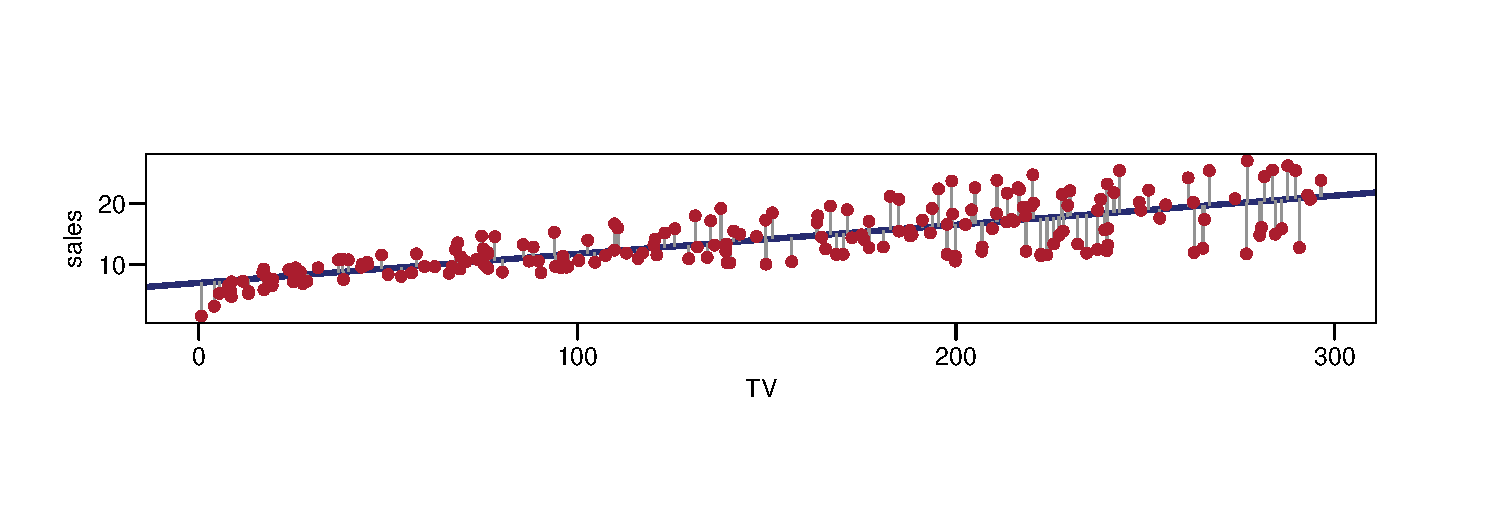
\includegraphics{Chapter3_files/figure-pdf/unnamed-chunk-8-1.pdf}

}

\caption{For the advertising data, the least squares fit for the
regression of sales onto TV. The fit is found by minimizing the sum of
squared errors. Each grey line segment represents an error, adn the fit
make a comprimise by averaging their squares. In this case a linear fit
captures the essence of the relationship, although it is somewhat
deficient in the left of the plot}

\end{figure}

So we have

\[
\hat{y_i} = 7.032 + 0.0475x_i
\]

According to this approximation an additional \$1,000 spent on TV
increases sales by 47.5 units.

\hypertarget{assessing-the-accuracy-of-the-coefficient-estimates}{%
\subsection{Assessing the Accuracy of the Coefficient
Estimates}\label{assessing-the-accuracy-of-the-coefficient-estimates}}

We assumed that \emph{true} relationship is linear:
\(Y = f(X) + \epsilon\). We don't know \(f\), and \(\epsilon\) is a
mean-zero random error term.

We said \(f\) is approximatly linear, so that
\(f(X) = \beta_0 + \beta_1 X\); which means

\[
Y = \beta_0 + \beta_1 X + \epsilon
\] (3.5)

error term captures: * the true relationship may not be linear * other
variables that affect Y * measurement error

and is independent of \(X\).

(3.5) is the \emph{population regression line}: the best linar
approximation to the true relationship between \(X\) and \(Y\).

\[
\hat{y} = \hat{\beta_0} + \hat{\beta_1}X
\] is the \emph{least squares line}. They are different of course! But
we don't know the population regression line. If we did:

For example, lets create a data;

\begin{itemize}
\tightlist
\item
  First we create random x values from 100 random numbers
\end{itemize}

\begin{Shaded}
\begin{Highlighting}[]
\FunctionTok{seq}\NormalTok{(}\SpecialCharTok{{-}}\DecValTok{2}\NormalTok{,}\DecValTok{2}\NormalTok{,}\AttributeTok{length.out=}\DecValTok{100}\NormalTok{)[}\DecValTok{1}\SpecialCharTok{:}\DecValTok{10}\NormalTok{]}
\end{Highlighting}
\end{Shaded}

\begin{verbatim}
 [1] -2.000000 -1.959596 -1.919192 -1.878788 -1.838384 -1.797980 -1.757576
 [8] -1.717172 -1.676768 -1.636364
\end{verbatim}

\begin{Shaded}
\begin{Highlighting}[]
\FunctionTok{set.seed}\NormalTok{(}\DecValTok{11}\NormalTok{)}
\NormalTok{x }\OtherTok{=} \FunctionTok{sample}\NormalTok{(}\FunctionTok{seq}\NormalTok{(}\SpecialCharTok{{-}}\DecValTok{2}\NormalTok{,}\DecValTok{2}\NormalTok{,}\AttributeTok{length.out =} \DecValTok{100}\NormalTok{),}\AttributeTok{size =} \DecValTok{100}\NormalTok{, }\AttributeTok{replace =}\NormalTok{ T)}
\NormalTok{x[}\DecValTok{1}\SpecialCharTok{:}\DecValTok{10}\NormalTok{]}
\end{Highlighting}
\end{Shaded}

\begin{verbatim}
 [1] -0.6666667  0.2222222 -1.0303030 -1.3939394 -0.5454545  0.3838384
 [7] -1.5555556  1.3939394  1.4343434  0.4646465
\end{verbatim}

lets define our \(f\)--population parameters \(\beta_0\) and \(\beta_1\)

\[
f(X) = 2 + 3\times X
\] Now lets create our \(Y\) values from this function but we also want
to add random error values as well

\begin{Shaded}
\begin{Highlighting}[]
\FunctionTok{set.seed}\NormalTok{(}\DecValTok{11}\NormalTok{)}
\NormalTok{y }\OtherTok{=} \DecValTok{2} \SpecialCharTok{+} \DecValTok{3}\SpecialCharTok{*}\NormalTok{x }\SpecialCharTok{+} \FunctionTok{rnorm}\NormalTok{(}\DecValTok{100}\NormalTok{)}
\NormalTok{y[}\DecValTok{1}\SpecialCharTok{:}\DecValTok{10}\NormalTok{]}
\end{Highlighting}
\end{Shaded}

\begin{verbatim}
 [1] -0.5910311  2.6932610 -2.6074622 -3.5444715  1.5421255  2.2173638
 [7] -1.3430610  6.8067360  6.2573073  2.3898188
\end{verbatim}

So we have a data set

\begin{Shaded}
\begin{Highlighting}[]
\NormalTok{data }\OtherTok{=} \FunctionTok{tibble}\NormalTok{(}
  \AttributeTok{y =}\NormalTok{ y, }\AttributeTok{x =}\NormalTok{ x}
\NormalTok{)}
\end{Highlighting}
\end{Shaded}

Now lets plot this data points

\begin{Shaded}
\begin{Highlighting}[]
\NormalTok{data }\SpecialCharTok{\%\textgreater{}\%} 
  \FunctionTok{ggplot}\NormalTok{() }\SpecialCharTok{+} \FunctionTok{aes}\NormalTok{(}\AttributeTok{x=}\NormalTok{x, }\AttributeTok{y=}\NormalTok{y) }\SpecialCharTok{+} \FunctionTok{geom\_point}\NormalTok{() }\SpecialCharTok{+} \FunctionTok{theme\_par}\NormalTok{()}
\end{Highlighting}
\end{Shaded}

\begin{figure}[H]

{\centering 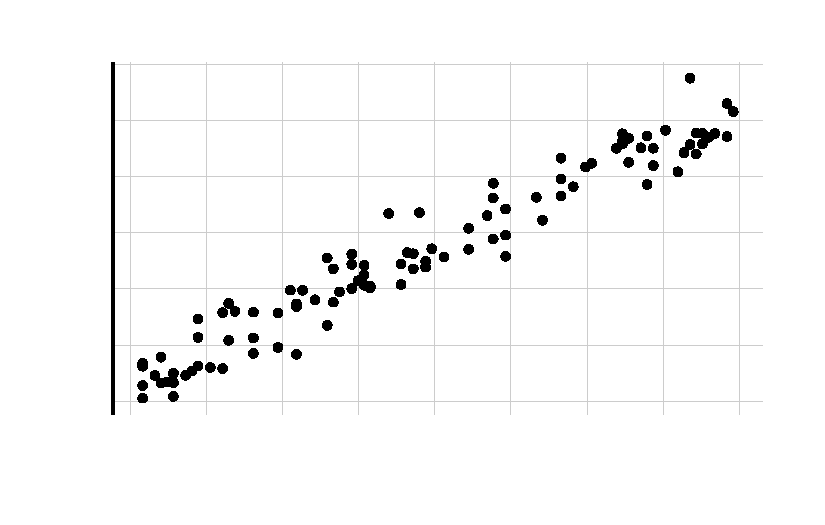
\includegraphics{Chapter3_files/figure-pdf/unnamed-chunk-13-1.pdf}

}

\end{figure}

Now, even though we already know \(f\) and population parameters
\(\beta_0 = 2\) and \(\beta_1 = 3\), lets estimate them:

\begin{Shaded}
\begin{Highlighting}[]
\FunctionTok{summary}\NormalTok{(}\FunctionTok{lm}\NormalTok{(y }\SpecialCharTok{\textasciitilde{}}\NormalTok{ x, }\AttributeTok{data =}\NormalTok{ data))}
\end{Highlighting}
\end{Shaded}

\begin{verbatim}

Call:
lm(formula = y ~ x, data = data)

Residuals:
     Min       1Q   Median       3Q      Max 
-2.01398 -0.65163 -0.06344  0.60455  2.39869 

Coefficients:
            Estimate Std. Error t value Pr(>|t|)    
(Intercept)  1.88077    0.09180   20.49   <2e-16 ***
x            3.05893    0.07608   40.20   <2e-16 ***
---
Signif. codes:  0 '***' 0.001 '**' 0.01 '*' 0.05 '.' 0.1 ' ' 1

Residual standard error: 0.9163 on 98 degrees of freedom
Multiple R-squared:  0.9428,    Adjusted R-squared:  0.9423 
F-statistic:  1616 on 1 and 98 DF,  p-value: < 2.2e-16
\end{verbatim}

So our \emph{least squares estimation is}

\[
\hat{y_i} = 1.88 + 3.06 x_i
\] Lets draw this \emph{least squares regression line to our plot}

\begin{Shaded}
\begin{Highlighting}[]
\NormalTok{data }\SpecialCharTok{\%\textgreater{}\%} 
  \FunctionTok{ggplot}\NormalTok{() }\SpecialCharTok{+} \FunctionTok{aes}\NormalTok{(}\AttributeTok{x=}\NormalTok{x, }\AttributeTok{y=}\NormalTok{y) }\SpecialCharTok{+} \FunctionTok{geom\_point}\NormalTok{() }\SpecialCharTok{+} \FunctionTok{geom\_abline}\NormalTok{(}\AttributeTok{intercept=}\FloatTok{1.88}\NormalTok{, }\AttributeTok{slope =} \FloatTok{3.06}\NormalTok{, }\AttributeTok{size =} \FloatTok{1.2}\NormalTok{) }\SpecialCharTok{+} \FunctionTok{theme\_par}\NormalTok{()}
\end{Highlighting}
\end{Shaded}

\begin{figure}[H]

{\centering 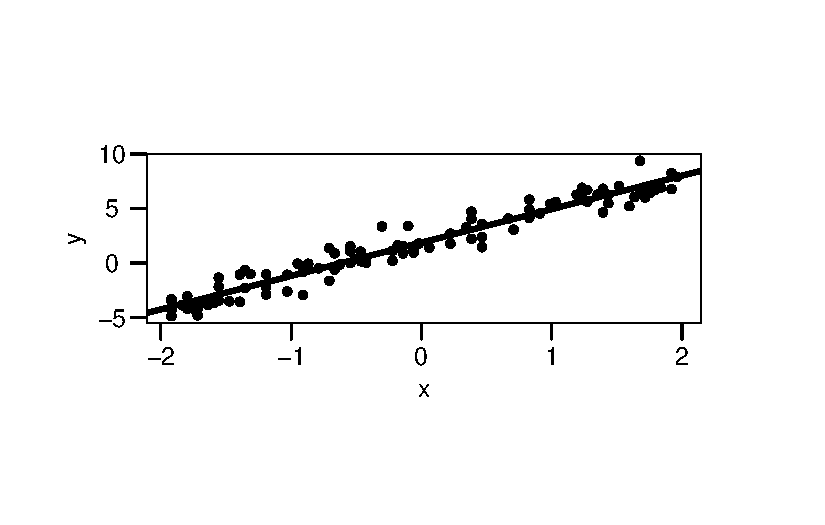
\includegraphics{Chapter3_files/figure-pdf/unnamed-chunk-15-1.pdf}

}

\end{figure}

What about the population regression line

\begin{Shaded}
\begin{Highlighting}[]
\NormalTok{data }\SpecialCharTok{\%\textgreater{}\%} 
  \FunctionTok{ggplot}\NormalTok{() }\SpecialCharTok{+} \FunctionTok{aes}\NormalTok{(}\AttributeTok{x=}\NormalTok{x, }\AttributeTok{y=}\NormalTok{y) }\SpecialCharTok{+} \FunctionTok{geom\_point}\NormalTok{() }\SpecialCharTok{+} \FunctionTok{geom\_abline}\NormalTok{(}\AttributeTok{intercept =} \FloatTok{1.9}\NormalTok{, }\AttributeTok{slope =} \FloatTok{3.06}\NormalTok{, }\AttributeTok{size =} \FloatTok{1.2}\NormalTok{) }\SpecialCharTok{+} \FunctionTok{geom\_abline}\NormalTok{(}\AttributeTok{intercept =} \DecValTok{2}\NormalTok{, }\AttributeTok{slope =} \DecValTok{3}\NormalTok{, }\AttributeTok{color =}\StringTok{"red"}\NormalTok{) }\SpecialCharTok{+} \FunctionTok{theme\_par}\NormalTok{()}
\end{Highlighting}
\end{Shaded}

\begin{figure}[H]

{\centering 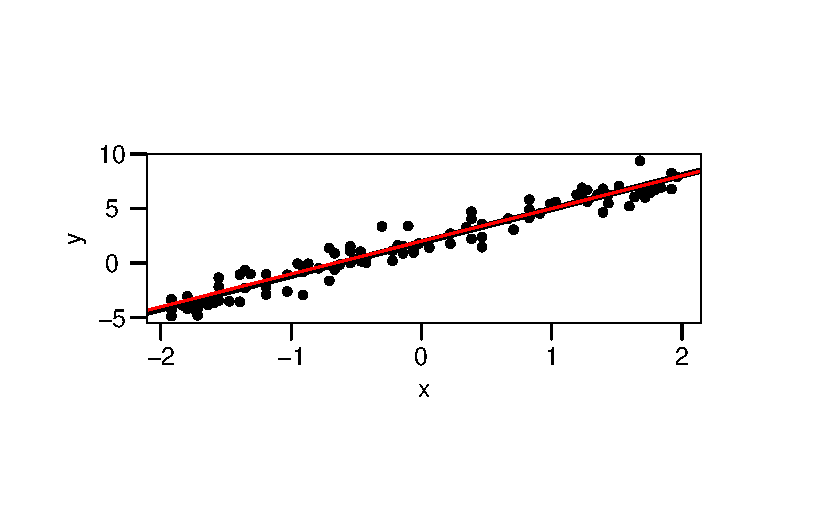
\includegraphics{Chapter3_files/figure-pdf/unnamed-chunk-16-1.pdf}

}

\end{figure}

They are not the same! If we were to have another data from the same
data generation process other estimates of parameters would result with
different \emph{least squares regression lines}:

\begin{Shaded}
\begin{Highlighting}[]
\FunctionTok{set.seed}\NormalTok{(}\DecValTok{111}\NormalTok{)}
\NormalTok{x\_r1 }\OtherTok{=} \FunctionTok{sample}\NormalTok{(}\FunctionTok{seq}\NormalTok{(}\SpecialCharTok{{-}}\DecValTok{2}\NormalTok{,}\DecValTok{2}\NormalTok{,}\AttributeTok{length.out =} \DecValTok{100}\NormalTok{),}\AttributeTok{size =} \DecValTok{100}\NormalTok{, }\AttributeTok{replace =}\NormalTok{ T)}
\NormalTok{y\_r1 }\OtherTok{=} \DecValTok{2} \SpecialCharTok{+} \DecValTok{3}\SpecialCharTok{*}\NormalTok{x\_r1 }\SpecialCharTok{+} \FunctionTok{rnorm}\NormalTok{(}\DecValTok{100}\NormalTok{)}
\FunctionTok{set.seed}\NormalTok{(}\DecValTok{1111}\NormalTok{)}
\NormalTok{x\_r2 }\OtherTok{=} \FunctionTok{sample}\NormalTok{(}\FunctionTok{seq}\NormalTok{(}\SpecialCharTok{{-}}\DecValTok{2}\NormalTok{,}\DecValTok{2}\NormalTok{,}\AttributeTok{length.out =} \DecValTok{100}\NormalTok{),}\AttributeTok{size =} \DecValTok{100}\NormalTok{, }\AttributeTok{replace =}\NormalTok{ T)}
\NormalTok{y\_r2 }\OtherTok{=} \DecValTok{2} \SpecialCharTok{+} \DecValTok{3}\SpecialCharTok{*}\NormalTok{x\_r2 }\SpecialCharTok{+} \FunctionTok{rnorm}\NormalTok{(}\DecValTok{100}\NormalTok{)}
\FunctionTok{set.seed}\NormalTok{(}\DecValTok{11111}\NormalTok{)}
\NormalTok{x\_r3 }\OtherTok{=} \FunctionTok{sample}\NormalTok{(}\FunctionTok{seq}\NormalTok{(}\SpecialCharTok{{-}}\DecValTok{2}\NormalTok{,}\DecValTok{2}\NormalTok{,}\AttributeTok{length.out =} \DecValTok{100}\NormalTok{),}\AttributeTok{size =} \DecValTok{100}\NormalTok{, }\AttributeTok{replace =}\NormalTok{ T)}
\NormalTok{y\_r3 }\OtherTok{=} \DecValTok{2} \SpecialCharTok{+} \DecValTok{3}\SpecialCharTok{*}\NormalTok{x\_r3 }\SpecialCharTok{+} \FunctionTok{rnorm}\NormalTok{(}\DecValTok{100}\NormalTok{)}
\FunctionTok{set.seed}\NormalTok{(}\DecValTok{111111}\NormalTok{)}
\NormalTok{x\_r4 }\OtherTok{=} \FunctionTok{sample}\NormalTok{(}\FunctionTok{seq}\NormalTok{(}\SpecialCharTok{{-}}\DecValTok{2}\NormalTok{,}\DecValTok{2}\NormalTok{,}\AttributeTok{length.out =} \DecValTok{100}\NormalTok{),}\AttributeTok{size =} \DecValTok{100}\NormalTok{, }\AttributeTok{replace =}\NormalTok{ T)}
\NormalTok{y\_r4 }\OtherTok{=} \DecValTok{2} \SpecialCharTok{+} \DecValTok{3}\SpecialCharTok{*}\NormalTok{x\_r4 }\SpecialCharTok{+} \FunctionTok{rnorm}\NormalTok{(}\DecValTok{100}\NormalTok{)}
\FunctionTok{set.seed}\NormalTok{(}\DecValTok{1111111}\NormalTok{)}
\NormalTok{x\_r5 }\OtherTok{=} \FunctionTok{sample}\NormalTok{(}\FunctionTok{seq}\NormalTok{(}\SpecialCharTok{{-}}\DecValTok{2}\NormalTok{,}\DecValTok{2}\NormalTok{,}\AttributeTok{length.out =} \DecValTok{100}\NormalTok{),}\AttributeTok{size =} \DecValTok{100}\NormalTok{, }\AttributeTok{replace =}\NormalTok{ T)}
\NormalTok{y\_r5 }\OtherTok{=} \DecValTok{2} \SpecialCharTok{+} \DecValTok{3}\SpecialCharTok{*}\NormalTok{x\_r5 }\SpecialCharTok{+} \FunctionTok{rnorm}\NormalTok{(}\DecValTok{100}\NormalTok{)}
\FunctionTok{set.seed}\NormalTok{(}\DecValTok{11111111}\NormalTok{)}
\NormalTok{x\_r6 }\OtherTok{=} \FunctionTok{sample}\NormalTok{(}\FunctionTok{seq}\NormalTok{(}\SpecialCharTok{{-}}\DecValTok{2}\NormalTok{,}\DecValTok{2}\NormalTok{,}\AttributeTok{length.out =} \DecValTok{100}\NormalTok{),}\AttributeTok{size =} \DecValTok{100}\NormalTok{, }\AttributeTok{replace =}\NormalTok{ T)}
\NormalTok{y\_r6 }\OtherTok{=} \DecValTok{2} \SpecialCharTok{+} \DecValTok{3}\SpecialCharTok{*}\NormalTok{x\_r6 }\SpecialCharTok{+} \FunctionTok{rnorm}\NormalTok{(}\DecValTok{100}\NormalTok{)}
\end{Highlighting}
\end{Shaded}

Lets now estimate population parameters for each of these data and plot
them

\begin{Shaded}
\begin{Highlighting}[]
\NormalTok{data\_r }\OtherTok{=} \FunctionTok{tibble}\NormalTok{(}
\NormalTok{  y\_r1,x\_r1,y\_r2,x\_r2,y\_r3,x\_r3,y\_r4,x\_r4, y\_r5,x\_r5,y\_r6,x\_r6}
\NormalTok{)}
\NormalTok{data\_r}
\end{Highlighting}
\end{Shaded}

\begin{verbatim}
# A tibble: 100 x 12
     y_r1   x_r1   y_r2    x_r2   y_r3   x_r3  y_r4   x_r4   y_r5    x_r5  y_r6
    <dbl>  <dbl>  <dbl>   <dbl>  <dbl>  <dbl> <dbl>  <dbl>  <dbl>   <dbl> <dbl>
 1  5.99   1.11   0.807 -0.263   8.82   1.80  -3.05 -1.52   7.64   1.68   6.49 
 2  6.53   1.35   3.74   0.141   6.23   1.92   5.11  1.27   8.71   2      7.75 
 3  6.28   1.31   2.16  -0.0202 -0.272 -0.707  2.39 -0.101  4.59   0.909  1.21 
 4  1.52  -0.141 -0.178 -0.990   5.45   0.788 -4.55 -1.84  -1.41  -1.11   0.478
 5  0.708 -1.03  -0.464 -0.586   0.361 -0.343 -3.31 -1.15   9.59   1.88   2.64 
 6  2.05   0.343  4.12   0.788  -1.09  -1.11  -5.13 -1.96   0.723 -0.586  4.10 
 7  4.54   0.747  5.44   1.60    0.479 -0.707  2.27  0.182  2.29  -0.263  3.68 
 8  1.69  -0.626  8.02   1.80   -2.23  -1.64   1.55  0.222 -1.45  -0.990  5.08 
 9  2.84   0.869  1.02   0.384   4.04   0.949  3.34 -0.747 -2.21  -0.828  8.33 
10 -0.933 -0.990  3.52   0.505  -0.471 -0.505 -1.07 -0.869  1.47   0.0606 2.45 
# i 90 more rows
# i 1 more variable: x_r6 <dbl>
\end{verbatim}

\begin{Shaded}
\begin{Highlighting}[]
\NormalTok{data }\SpecialCharTok{\%\textgreater{}\%} 
  \FunctionTok{ggplot}\NormalTok{() }\SpecialCharTok{+} \FunctionTok{aes}\NormalTok{(x,y) }\SpecialCharTok{+} \FunctionTok{geom\_point}\NormalTok{(}\AttributeTok{size =} \DecValTok{0}\NormalTok{, }\AttributeTok{color =} \StringTok{"white"}\NormalTok{)  }\SpecialCharTok{+} 
  \FunctionTok{geom\_abline}\NormalTok{(}\AttributeTok{intercept =} \FunctionTok{lm}\NormalTok{(y\_r1 }\SpecialCharTok{\textasciitilde{}}\NormalTok{ x\_r1)}\SpecialCharTok{$}\NormalTok{coefficients[}\DecValTok{1}\NormalTok{], }\AttributeTok{slope =} \FunctionTok{lm}\NormalTok{(y\_r1 }\SpecialCharTok{\textasciitilde{}}\NormalTok{ x\_r1)}\SpecialCharTok{$}\NormalTok{coefficients[}\DecValTok{2}\NormalTok{], }\AttributeTok{color =}\StringTok{"\#29019F"}\NormalTok{) }\SpecialCharTok{+}
  \FunctionTok{geom\_abline}\NormalTok{(}\AttributeTok{intercept =} \FunctionTok{lm}\NormalTok{(y\_r2 }\SpecialCharTok{\textasciitilde{}}\NormalTok{ x\_r2)}\SpecialCharTok{$}\NormalTok{coefficients[}\DecValTok{1}\NormalTok{], }\AttributeTok{slope =} \FunctionTok{lm}\NormalTok{(y\_r2 }\SpecialCharTok{\textasciitilde{}}\NormalTok{ x\_r2)}\SpecialCharTok{$}\NormalTok{coefficients[}\DecValTok{2}\NormalTok{], }\AttributeTok{color =}\StringTok{"\#0A04BF"}\NormalTok{) }\SpecialCharTok{+}
  \FunctionTok{geom\_abline}\NormalTok{(}\AttributeTok{intercept =} \FunctionTok{lm}\NormalTok{(y\_r3 }\SpecialCharTok{\textasciitilde{}}\NormalTok{ x\_r3)}\SpecialCharTok{$}\NormalTok{coefficients[}\DecValTok{1}\NormalTok{], }\AttributeTok{slope =} \FunctionTok{lm}\NormalTok{(y\_r3 }\SpecialCharTok{\textasciitilde{}}\NormalTok{ x\_r3)}\SpecialCharTok{$}\NormalTok{coefficients[}\DecValTok{2}\NormalTok{], }\AttributeTok{color =}\StringTok{"\#0930DF"}\NormalTok{) }\SpecialCharTok{+}
  \FunctionTok{geom\_abline}\NormalTok{(}\AttributeTok{intercept =} \FunctionTok{lm}\NormalTok{(y\_r4 }\SpecialCharTok{\textasciitilde{}}\NormalTok{ x\_r4)}\SpecialCharTok{$}\NormalTok{coefficients[}\DecValTok{1}\NormalTok{], }\AttributeTok{slope =} \FunctionTok{lm}\NormalTok{(y\_r4 }\SpecialCharTok{\textasciitilde{}}\NormalTok{ x\_r4)}\SpecialCharTok{$}\NormalTok{coefficients[}\DecValTok{2}\NormalTok{], }\AttributeTok{color =}\StringTok{"\#0E6DFF"}\NormalTok{) }\SpecialCharTok{+}
  \FunctionTok{geom\_abline}\NormalTok{(}\AttributeTok{intercept =} \FunctionTok{lm}\NormalTok{(y\_r5 }\SpecialCharTok{\textasciitilde{}}\NormalTok{ x\_r5)}\SpecialCharTok{$}\NormalTok{coefficients[}\DecValTok{1}\NormalTok{], }\AttributeTok{slope =} \FunctionTok{lm}\NormalTok{(y\_r5 }\SpecialCharTok{\textasciitilde{}}\NormalTok{ x\_r5)}\SpecialCharTok{$}\NormalTok{coefficients[}\DecValTok{2}\NormalTok{], }\AttributeTok{color =}\StringTok{"\#2BA8FF"}\NormalTok{) }\SpecialCharTok{+}
  \FunctionTok{geom\_abline}\NormalTok{(}\AttributeTok{intercept =} \FunctionTok{lm}\NormalTok{(y\_r6 }\SpecialCharTok{\textasciitilde{}}\NormalTok{ x\_r6)}\SpecialCharTok{$}\NormalTok{coefficients[}\DecValTok{1}\NormalTok{], }\AttributeTok{slope =} \FunctionTok{lm}\NormalTok{(y\_r6 }\SpecialCharTok{\textasciitilde{}}\NormalTok{ x\_r6)}\SpecialCharTok{$}\NormalTok{coefficients[}\DecValTok{2}\NormalTok{], }\AttributeTok{color =}\StringTok{"\#48D9FF"}\NormalTok{) }\SpecialCharTok{+}
  \FunctionTok{geom\_abline}\NormalTok{(}\AttributeTok{intercept =}\DecValTok{2}\NormalTok{, }\AttributeTok{slope =}\DecValTok{3}\NormalTok{, }\AttributeTok{color =} \StringTok{"red"}\NormalTok{) }\SpecialCharTok{+}
  
  \FunctionTok{theme\_par}\NormalTok{()}
\end{Highlighting}
\end{Shaded}

\begin{figure}[H]

{\centering 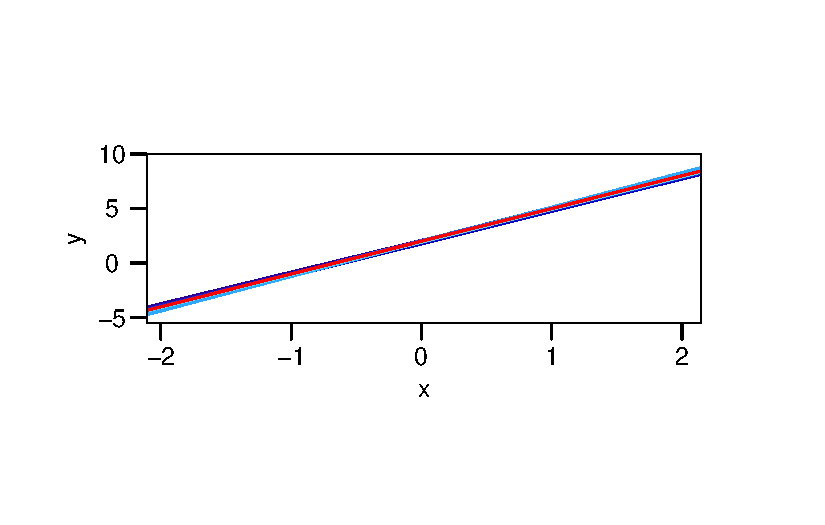
\includegraphics{Chapter3_files/figure-pdf/unnamed-chunk-19-1.pdf}

}

\end{figure}

So, different data sets generated from the same true model result in
slightly different least squares lines, but the unobserved population
regression line does not change.

This is because we are using a sample, and estimating characteristics of
the population. Usually these characteristics are different, but
generally sample characteristics will provide a good estimate to the
population characteristics.

Computing \(\hat{\beta_0}\) and \(\hat{\beta_1}\) from different sets of
sample data provide different but similar results. And we are trying to
estimate population parameters \(\beta_0\) and \(\beta_1\) with these.
Some of these \(\hat{\beta_0}\) and \(\hat{\beta_1}\) will overestimate,
some will underestimate \(\beta_0\), and \(\beta_1\). But if we could
average all these estimated parameters and take the average, than this
average should be equal to population parameters; if this is the case
this estimator is called \emph{unbiased estimator}. So an unbiased
estimator does not \emph{systematically} over- or under-estimate the
true parameter.

Okay but how close \(\hat{\beta_0}\) and \(\hat{\beta_1}\) are to the
true values \(\beta_0\) and \(\beta_1\). We want to compute the standard
errors associated with \(\hat{\beta_0}\) and \(\hat{\beta_1}\). Standard
error telss us the average amount of estimate differes from the actual
value.

\[
\begin{align}
\text{SE}(\hat{\beta_0})^2 &= \sigma^2 \left[\frac{1}{n} + \frac{\bar{x}^2}{\sum_{i=1}^n(x_i - \bar{x}^2)}\right] \\
\text{SE}(\hat{\beta_1})^2 &= \frac{\sigma^2}{\sum_{i=1}^n(x_i-\bar{x})^2}
\end{align}
\] (3.8)

Where \(\sigma^2=\text{Var}(\epsilon)\).

Notice that formula of \(\text{SE}(\hat{\beta_1})\) is smaller when
\(x_i\) are more spread out; intutively we have more \emph{leverage} to
estimate a slope when this is the case.

In general \(\sigma^2\) is not known, but can be estimated from the
data. The estimate of \(\sigma\) is known as the \emph{residual standard
error}, and given by the formula

\[
\text{RSE} = \sqrt{\text{RSS}/(n-2)}
\] So, when \(\sigma^2\) is estimated fro mthe data we should write
\(\hat{\text{SE}}(\hat{\beta_1})\) to indicate that an estimate has been
made, but usually we drop this extra hat.

Standard errors can be used to compute \emph{confidence intervals}. A
95\% confidence interval is defines as a range of values such that with
95\% probability, the rage will contain the true unknown value of the
parameter. The range is defined in terms of lower and upper limits
computed from the sample of data. For linear regression, the 95\%
confidence interval for \(\beta_1\) approximately takes the form

\[
\hat{\beta_1} \pm 1.96 \cdot \text{SE}(\hat{\beta_1}) 
\] (3.9)

So there is approximately a 95\% chance that the interval
\[[\hat{\beta_1} - 1.96 \cdot \text{SE}(\hat{\beta_1}), \hat{\beta_1} + 1.96 \cdot \text{SE}(\hat{\beta-1})]\]
(3.10) will contain the true value of \(\beta_1\). Same is true for
\(\beta_0\)

\[
\hat{\beta_0} \pm 1.96 \cdot \text{SE}(\hat{\beta_0})
\] (3.11)

Lets calculate the confidence intervals for \(\beta_0\) and \(\beta_1\)
from our original data and model

\[
\hat{sales_i} = \hat{\beta_0} + \hat{\beta_1}\cdot TV
\] We first need to calculate RSS and RSE:

\[
\text{RSS} = \sum(y_i - \hat{y_i})^2
\]

\begin{Shaded}
\begin{Highlighting}[]
\NormalTok{RSS }\OtherTok{=} \FunctionTok{sum}\NormalTok{((advertising}\SpecialCharTok{$}\NormalTok{sales }\SpecialCharTok{{-}}\NormalTok{ y\_hat\_adv)}\SpecialCharTok{\^{}}\DecValTok{2}\NormalTok{)}
\NormalTok{RSS}
\end{Highlighting}
\end{Shaded}

\begin{verbatim}
[1] 2102.531
\end{verbatim}

\[
\text{RSE} = \sigma = \sqrt{RSS/(n-2)}
\]

\begin{Shaded}
\begin{Highlighting}[]
\NormalTok{RSE }\OtherTok{=} \FunctionTok{sqrt}\NormalTok{((RSS }\SpecialCharTok{/}\NormalTok{ (}\FunctionTok{length}\NormalTok{(advertising}\SpecialCharTok{$}\NormalTok{sales) }\SpecialCharTok{{-}}\DecValTok{2}\NormalTok{)))}
\NormalTok{RSE}
\end{Highlighting}
\end{Shaded}

\begin{verbatim}
[1] 3.258656
\end{verbatim}

For \(\beta_0\)

\[
\text{SE}(\hat{\beta_0}) = \sigma^2 \left[\frac{1}{n} + \frac{\bar{x}^2}{\sum_{i=1}^n(x_i - \bar{x})^2} \right]
\]

\begin{Shaded}
\begin{Highlighting}[]
\NormalTok{se\_beta\_0\_adv }\OtherTok{=}  \FunctionTok{sqrt}\NormalTok{(RSE}\SpecialCharTok{\^{}}\DecValTok{2} \SpecialCharTok{*}\NormalTok{ (}\DecValTok{1}\SpecialCharTok{/}\FunctionTok{length}\NormalTok{(advertising}\SpecialCharTok{$}\NormalTok{sales) }\SpecialCharTok{+}\NormalTok{ (}\FunctionTok{mean}\NormalTok{(advertising}\SpecialCharTok{$}\NormalTok{TV)}\SpecialCharTok{\^{}}\DecValTok{2} \SpecialCharTok{/} \FunctionTok{sum}\NormalTok{((advertising}\SpecialCharTok{$}\NormalTok{TV }\SpecialCharTok{{-}} \FunctionTok{mean}\NormalTok{(advertising}\SpecialCharTok{$}\NormalTok{TV))}\SpecialCharTok{\^{}}\DecValTok{2}\NormalTok{))))}
\NormalTok{se\_beta\_0\_adv}
\end{Highlighting}
\end{Shaded}

\begin{verbatim}
[1] 0.4578429
\end{verbatim}

So we can calculate the confidence interval for \(\beta_0\)

\begin{Shaded}
\begin{Highlighting}[]
\FunctionTok{cat}\NormalTok{(}\StringTok{"In the absence of any advertising, sales will on average, fall somewhere between"}\NormalTok{,beta\_0\_hat\_adv }\SpecialCharTok{{-}} \FloatTok{1.96} \SpecialCharTok{*}\NormalTok{ se\_beta\_0\_adv, }\StringTok{"and"}\NormalTok{, beta\_0\_hat\_adv }\SpecialCharTok{+} \FloatTok{1.96} \SpecialCharTok{*}\NormalTok{ se\_beta\_0\_adv)}
\end{Highlighting}
\end{Shaded}

\begin{verbatim}
In the absence of any advertising, sales will on average, fall somewhere between 6.135221 and 7.929966
\end{verbatim}

For \(\hat{\beta_1}\):

\[
\text{SE}(\hat{\beta_1})^2 =\frac{\sigma^2}{\sum(x_i - \bar{x})^2}
\]

\begin{Shaded}
\begin{Highlighting}[]
\NormalTok{se\_beta\_1\_adv }\OtherTok{=} \FunctionTok{sqrt}\NormalTok{(RSE}\SpecialCharTok{\^{}}\DecValTok{2} \SpecialCharTok{/}\NormalTok{ (}\FunctionTok{sum}\NormalTok{((advertising}\SpecialCharTok{$}\NormalTok{TV }\SpecialCharTok{{-}} \FunctionTok{mean}\NormalTok{(advertising}\SpecialCharTok{$}\NormalTok{TV))}\SpecialCharTok{\^{}}\DecValTok{2}\NormalTok{)))}
\NormalTok{se\_beta\_1\_adv}
\end{Highlighting}
\end{Shaded}

\begin{verbatim}
[1] 0.002690607
\end{verbatim}

\begin{Shaded}
\begin{Highlighting}[]
\FunctionTok{cat}\NormalTok{(}\StringTok{"For each $1,000 increase in TV advertising, average increase in sales will be between"}\NormalTok{,(beta\_1\_hat\_adv }\SpecialCharTok{{-}} \FloatTok{1.96} \SpecialCharTok{*}\NormalTok{ se\_beta\_1\_adv) }\SpecialCharTok{*} \DecValTok{1000}\NormalTok{, }\StringTok{"and"}\NormalTok{, (beta\_1\_hat\_adv }\SpecialCharTok{+} \FloatTok{1.96} \SpecialCharTok{*}\NormalTok{ se\_beta\_1\_adv)}\SpecialCharTok{*}\DecValTok{1000}\NormalTok{, }\StringTok{"by 95\% confidence"}\NormalTok{)}
\end{Highlighting}
\end{Shaded}

\begin{verbatim}
For each $1,000 increase in TV advertising, average increase in sales will be between 42.26305 and 52.81023 by 95% confidence
\end{verbatim}

Lets confirm our results

\begin{Shaded}
\begin{Highlighting}[]
\FunctionTok{summary}\NormalTok{(}\FunctionTok{lm}\NormalTok{(sales }\SpecialCharTok{\textasciitilde{}}\NormalTok{ TV, advertising))}
\end{Highlighting}
\end{Shaded}

\begin{verbatim}

Call:
lm(formula = sales ~ TV, data = advertising)

Residuals:
    Min      1Q  Median      3Q     Max 
-8.3860 -1.9545 -0.1913  2.0671  7.2124 

Coefficients:
            Estimate Std. Error t value Pr(>|t|)    
(Intercept) 7.032594   0.457843   15.36   <2e-16 ***
TV          0.047537   0.002691   17.67   <2e-16 ***
---
Signif. codes:  0 '***' 0.001 '**' 0.01 '*' 0.05 '.' 0.1 ' ' 1

Residual standard error: 3.259 on 198 degrees of freedom
Multiple R-squared:  0.6119,    Adjusted R-squared:  0.6099 
F-statistic: 312.1 on 1 and 198 DF,  p-value: < 2.2e-16
\end{verbatim}

\begin{Shaded}
\begin{Highlighting}[]
\FunctionTok{confint}\NormalTok{(}\FunctionTok{lm}\NormalTok{(sales }\SpecialCharTok{\textasciitilde{}}\NormalTok{ TV, advertising))}
\end{Highlighting}
\end{Shaded}

\begin{verbatim}
                 2.5 %     97.5 %
(Intercept) 6.12971927 7.93546783
TV          0.04223072 0.05284256
\end{verbatim}

So standard errors of our estimated parameters tells us the average
amount of difference from the true population parameters. And using the
confidence intervals we can tell a range of the true population
parameters' interval with a percentage (usually 95\%).

Lets do this for our \texttt{data} as well, which we know has the form

\[
y_i = 2 + 3 x_i + \epsilon_i
\] Lets calculate \(\hat{\beta_0}\) and \(\hat{\beta_1}\) first

\begin{Shaded}
\begin{Highlighting}[]
\NormalTok{beta\_1\_hat\_data }\OtherTok{=} \FunctionTok{sum}\NormalTok{((data}\SpecialCharTok{$}\NormalTok{x }\SpecialCharTok{{-}} \FunctionTok{mean}\NormalTok{(data}\SpecialCharTok{$}\NormalTok{x)) }\SpecialCharTok{*}\NormalTok{ (data}\SpecialCharTok{$}\NormalTok{y }\SpecialCharTok{{-}} \FunctionTok{mean}\NormalTok{(data}\SpecialCharTok{$}\NormalTok{y))) }\SpecialCharTok{/} \FunctionTok{sum}\NormalTok{((data}\SpecialCharTok{$}\NormalTok{x }\SpecialCharTok{{-}} \FunctionTok{mean}\NormalTok{(data}\SpecialCharTok{$}\NormalTok{x))}\SpecialCharTok{\^{}}\DecValTok{2}\NormalTok{)}
\NormalTok{beta\_1\_hat\_data}
\end{Highlighting}
\end{Shaded}

\begin{verbatim}
[1] 3.058925
\end{verbatim}

\begin{Shaded}
\begin{Highlighting}[]
\NormalTok{beta\_0\_hat\_data }\OtherTok{=} \FunctionTok{mean}\NormalTok{(data}\SpecialCharTok{$}\NormalTok{y) }\SpecialCharTok{{-}}\NormalTok{ beta\_1\_hat\_data }\SpecialCharTok{*} \FunctionTok{mean}\NormalTok{(data}\SpecialCharTok{$}\NormalTok{x)}
\NormalTok{beta\_0\_hat\_data}
\end{Highlighting}
\end{Shaded}

\begin{verbatim}
[1] 1.880772
\end{verbatim}

\[
\hat{y_i} = 1.88 + 3.05 x_i
\]

lets confirm this

\begin{Shaded}
\begin{Highlighting}[]
\FunctionTok{lm}\NormalTok{(y}\SpecialCharTok{\textasciitilde{}}\NormalTok{x, data)}
\end{Highlighting}
\end{Shaded}

\begin{verbatim}

Call:
lm(formula = y ~ x, data = data)

Coefficients:
(Intercept)            x  
      1.881        3.059  
\end{verbatim}

Lets calculate the residual sum of squares, residual sum of errors,
standard errors, and confidence intervals

\begin{Shaded}
\begin{Highlighting}[]
\NormalTok{data }\SpecialCharTok{\%\textgreater{}\%} 
  \FunctionTok{mutate}\NormalTok{(}
    \AttributeTok{y\_hat =}\NormalTok{ beta\_0\_hat\_data }\SpecialCharTok{+}\NormalTok{ beta\_1\_hat\_data }\SpecialCharTok{*}\NormalTok{ x}
\NormalTok{  ) }\OtherTok{{-}\textgreater{}}\NormalTok{ data}
\end{Highlighting}
\end{Shaded}

\begin{Shaded}
\begin{Highlighting}[]
\NormalTok{RSS\_data }\OtherTok{=} \FunctionTok{sum}\NormalTok{((data}\SpecialCharTok{$}\NormalTok{y }\SpecialCharTok{{-}}\NormalTok{ data}\SpecialCharTok{$}\NormalTok{y\_hat)}\SpecialCharTok{\^{}}\DecValTok{2}\NormalTok{)}
\NormalTok{RSS\_data}
\end{Highlighting}
\end{Shaded}

\begin{verbatim}
[1] 82.28514
\end{verbatim}

\begin{Shaded}
\begin{Highlighting}[]
\NormalTok{RSE\_data }\OtherTok{=} \FunctionTok{sqrt}\NormalTok{((RSS\_data}\SpecialCharTok{/}\NormalTok{(}\FunctionTok{length}\NormalTok{(data}\SpecialCharTok{$}\NormalTok{y) }\SpecialCharTok{{-}}\DecValTok{2}\NormalTok{)))}
\NormalTok{RSE\_data}
\end{Highlighting}
\end{Shaded}

\begin{verbatim}
[1] 0.9163211
\end{verbatim}

so \(\sigma_{data} = 0.9163\)

We can now compute the standard errors of estiamed coefficients

\begin{Shaded}
\begin{Highlighting}[]
\NormalTok{se\_beta\_0\_data }\OtherTok{=} \FunctionTok{sqrt}\NormalTok{(((}\DecValTok{1}\SpecialCharTok{/}\FunctionTok{length}\NormalTok{(data}\SpecialCharTok{$}\NormalTok{y)) }\SpecialCharTok{+}\NormalTok{ (}\FunctionTok{mean}\NormalTok{(data}\SpecialCharTok{$}\NormalTok{x)}\SpecialCharTok{\^{}}\DecValTok{2} \SpecialCharTok{/} \FunctionTok{sum}\NormalTok{((data}\SpecialCharTok{$}\NormalTok{x }\SpecialCharTok{{-}} \FunctionTok{mean}\NormalTok{(data}\SpecialCharTok{$}\NormalTok{x))}\SpecialCharTok{\^{}}\DecValTok{2}\NormalTok{))) }\SpecialCharTok{*}\NormalTok{ RSE\_data}\SpecialCharTok{\^{}}\DecValTok{2}\NormalTok{)}
\NormalTok{se\_beta\_0\_data}
\end{Highlighting}
\end{Shaded}

\begin{verbatim}
[1] 0.09179903
\end{verbatim}

\begin{Shaded}
\begin{Highlighting}[]
\NormalTok{se\_beta\_1\_data }\OtherTok{=} \FunctionTok{sqrt}\NormalTok{(RSE\_data}\SpecialCharTok{\^{}}\DecValTok{2} \SpecialCharTok{/}\NormalTok{ (}\FunctionTok{sum}\NormalTok{((data}\SpecialCharTok{$}\NormalTok{x }\SpecialCharTok{{-}} \FunctionTok{mean}\NormalTok{(data}\SpecialCharTok{$}\NormalTok{x))}\SpecialCharTok{\^{}}\DecValTok{2}\NormalTok{)))}
\NormalTok{se\_beta\_1\_data}
\end{Highlighting}
\end{Shaded}

\begin{verbatim}
[1] 0.07608457
\end{verbatim}

Lets confirm

\begin{Shaded}
\begin{Highlighting}[]
\FunctionTok{summary}\NormalTok{(}\FunctionTok{lm}\NormalTok{(y}\SpecialCharTok{\textasciitilde{}}\NormalTok{x,data))}
\end{Highlighting}
\end{Shaded}

\begin{verbatim}

Call:
lm(formula = y ~ x, data = data)

Residuals:
     Min       1Q   Median       3Q      Max 
-2.01398 -0.65163 -0.06344  0.60455  2.39869 

Coefficients:
            Estimate Std. Error t value Pr(>|t|)    
(Intercept)  1.88077    0.09180   20.49   <2e-16 ***
x            3.05893    0.07608   40.20   <2e-16 ***
---
Signif. codes:  0 '***' 0.001 '**' 0.01 '*' 0.05 '.' 0.1 ' ' 1

Residual standard error: 0.9163 on 98 degrees of freedom
Multiple R-squared:  0.9428,    Adjusted R-squared:  0.9423 
F-statistic:  1616 on 1 and 98 DF,  p-value: < 2.2e-16
\end{verbatim}

So we can say that on average our \(\hat{\beta_0}\)s are 0.091 differ
from \(\beta_0\), and our \(\hat{\beta_1}\)s differ 0.076 from
\(\beta_1\). To make more sense of it we can calculate the confidence
intervals

\begin{Shaded}
\begin{Highlighting}[]
\FunctionTok{cat}\NormalTok{(}\StringTok{"By 95\% confidence we can say that the true beta\_0 is between"}\NormalTok{, beta\_0\_hat\_data }\SpecialCharTok{{-}} \FloatTok{1.96} \SpecialCharTok{*}\NormalTok{ se\_beta\_0\_data, }\StringTok{"and"}\NormalTok{, beta\_0\_hat\_data }\SpecialCharTok{+} \FloatTok{1.96} \SpecialCharTok{*}\NormalTok{ se\_beta\_0\_data )}
\end{Highlighting}
\end{Shaded}

\begin{verbatim}
By 95% confidence we can say that the true beta_0 is between 1.700846 and 2.060698
\end{verbatim}

\begin{Shaded}
\begin{Highlighting}[]
\FunctionTok{cat}\NormalTok{(}\StringTok{"By 95\% confidence we can say that the true beta\_0 is between"}\NormalTok{, beta\_1\_hat\_data }\SpecialCharTok{{-}} \FloatTok{1.96} \SpecialCharTok{*}\NormalTok{ se\_beta\_1\_data, }\StringTok{"and"}\NormalTok{, beta\_1\_hat\_data }\SpecialCharTok{+} \FloatTok{1.96} \SpecialCharTok{*}\NormalTok{ se\_beta\_1\_data)}
\end{Highlighting}
\end{Shaded}

\begin{verbatim}
By 95% confidence we can say that the true beta_0 is between 2.909799 and 3.208051
\end{verbatim}

Lets confirm this

\begin{Shaded}
\begin{Highlighting}[]
\FunctionTok{confint}\NormalTok{(}\FunctionTok{lm}\NormalTok{(y}\SpecialCharTok{\textasciitilde{}}\NormalTok{x,data))}
\end{Highlighting}
\end{Shaded}

\begin{verbatim}
               2.5 %   97.5 %
(Intercept) 1.698600 2.062944
x           2.907938 3.209912
\end{verbatim}

Since standard error tells us the range of the \(\beta\) values via
confidence interval, we can infer that if this range does not include 0,
than our \(\beta\) values are statistically significant; x is assocaited
with y.

Or we can use standard erros to perform \emph{hypothesis tests} on the
coefficients. We usually don't care about the intercept, so lets do the
hypothesis test on only \(\hat{\beta_1}\).

\[
\begin{align}
H_0 &: \beta_1 = 0 \to \text{there is no relationship between X and Y} \\
H_1 &: \beta_1 \neq 0 \to \text{there is some relationship between X and Y}
\end{align}
\] If the \emph{null-hypothesis} is true =\textgreater{} \$ \beta\_1 =
0\$ =\textgreater{} \(Y = \beta_0 + \epsilon\) =\textgreater{} \(X\) is
not associated with \(Y\).

To test the null-hypothessi, we need to determine whether our estimate
\(\hat{\beta_1}\) is sufficiently far from zero that we can be confident
that \(\beta_1\) is non-zero. How far is enough? This depends on the
accuracy of \(\hat{\beta_1}\)--that is it depends on
\(\text{SE}(\hat{\beta_1})\). If \(\text{SE}(\hat{\beta_1})\) is small,
then even relatively small values of \(\hat{\beta_1}\) may provide
strong evidence that \(\beta_1 \neq 0\). If \(\text{SE}(\hat{\beta_1})\)
is large, then \(\hat{\beta_1}\) must be large in absolute value in
order for us to reject the null hypothessis. In practice we compute a
\emph{t-statistic} given by

\[
t = \frac{\hat{\beta_1} - 0}{\text{SE}(\hat{\beta_1})}
\] (3.14)

which measures the number of standard deviations that \(\hat{\beta_1}\)
is away from zero. From the t-statistic we can compute the
\emph{p-value}; a small p value indicates that it is unlikely to observe
such a substantial association between the predictor and the response
due to chance, in absence of any real association between the predictor
and the response. So if p value is small we infer that there is
assocaition between the predictor and the response =\textgreater{} we
reject the null hypothesis. Typical p-value cutoffs for rejecting the
null hypothesis are 5 or 1\%. When \(n=30\) these correspond to
tstatsitcs of around 2 and 2.75.

\begin{Shaded}
\begin{Highlighting}[]
\FunctionTok{summary}\NormalTok{(}\FunctionTok{lm}\NormalTok{(sales }\SpecialCharTok{\textasciitilde{}}\NormalTok{ TV, advertising))}
\end{Highlighting}
\end{Shaded}

\begin{verbatim}

Call:
lm(formula = sales ~ TV, data = advertising)

Residuals:
    Min      1Q  Median      3Q     Max 
-8.3860 -1.9545 -0.1913  2.0671  7.2124 

Coefficients:
            Estimate Std. Error t value Pr(>|t|)    
(Intercept) 7.032594   0.457843   15.36   <2e-16 ***
TV          0.047537   0.002691   17.67   <2e-16 ***
---
Signif. codes:  0 '***' 0.001 '**' 0.01 '*' 0.05 '.' 0.1 ' ' 1

Residual standard error: 3.259 on 198 degrees of freedom
Multiple R-squared:  0.6119,    Adjusted R-squared:  0.6099 
F-statistic: 312.1 on 1 and 198 DF,  p-value: < 2.2e-16
\end{verbatim}

Here we see that t statistics are very high, and p values are very low
=\textgreater{} reject the null hypothesis for both \(\beta\) values;
they are statistically significant.

\hypertarget{assessing-the-accuracy-of-the-model}{%
\subsection{Assessing the Accuracy of the
Model}\label{assessing-the-accuracy-of-the-model}}

Once we concluded the statistically significant variable--rejecting the
null hypothesis, we want to quantify \emph{the extend to which the model
fits the data}. We can use either

\begin{itemize}
\tightlist
\item
  \emph{Residual standard error}
\item
  \(R^2\)
\end{itemize}

\emph{Residual standard error}

Recall from \(Y_i = \beta_0 + \beta_1 X_i + \epsilon_i\) that associated
with each observation is an error term \(\epsilon\). Because of these
error terms even if we knew the true regression line, we would not be
able to predict \(Y\) from \(X\). The \emph{RSE} is an estimate of the
standard deviation of \(\epsilon\). It is the average amount that the
response will deviate from the true regression line, computed by

\[
\begin{align}
\text{RSE} &= \sqrt{\frac{1}{n-2}\text{RSS}} \\
&= \sqrt{\frac{1}{n-2}\sum_{i=1}^n(y_i - \hat{y_i})^2}
\end{align}
\] (3.15)

In the advertising data, RSE was 3.26; actual sales in each market
deviate from the true regression line by approximately 3,269 units, on
average. This also means that; if the model were correct and the true
values of the unknown coefficients \(\beta_0\) and \(\beta_1\) were
known exaclty, any predcition of sales on the basis of TV advertising
would still be off by about 3,260 units on average. Is this prediction
error accaptable? Depends on the data: in the \texttt{advertising} data
set the mean value of \texttt{sales} is \(\approx 14,000\) units, and so
the percentage error is \(3,260 / 14,000 = 23%
\).

The RSE is considered a measure of the \emph{lack of fit} of the model
\(Y=\beta_0 + \beta_1 + \epsilon\) to the data. If the predictions from
the model are very close to the true outcome
values--\(\hat{y_i} \approx y_i\) then RSE will be small, and we can
concldue that the model fits the data very well. Otherwise, if
\(\hat{y_i}\) is very far from \(y_i\) then RSE may be quite large,
indicating the model doesn't fit the data well.

\(R^2\)\textbf{Statistic}

The RSE provides an absolute measure of lack of fit of the model to the
data. \(R^2\) provides an alternative measure of fit. It takes the form
of a \emph{proportion}--the proportion of variance explained--and so its
always \(0\leq R^2 \leq 1\) and is independent of the scale of \(Y\)--as
opposed to RSE.

\[
R^2 = \frac{TSS - RSS}{TSS} = 1 - \frac{RSS}{TSS}
\] (3.17)

where \(\text{TSS} = \sum(y_i - \bar{y})^2\) is the \emph{total sun of
squares} and \(\text{RSS} = \sum(y_i - \hat{y_i})^2\). TSS measures the
total variaance in the response \(Y\); and can be thought of as the
amount of varaiblity ingerent in the response before the regression is
performed. RSS measures the amount of varaiblity that is left
unexplained after performing the regression. So TSS - RSS measures the
amount of variability in the response that is explained by performing
the regression, and \(R^2\) measures the \emph{proportion of variability
in} \(Y\) \emph{that can be explained using} \(X\). As \(R^2\) gets
closer to 1, a large proportion of the variability in the response has
been explained by the regression. A number near 0 indicates that the
regression did not explain much of the variablity in the response; this
might occur because the linear model is wrong, or the inherit error
\(\sigma^2 = \text{RSE}^2\) is high, or both.

Lets calculate \(R^2\) of our estimation on \texttt{advertising} data
with the model \(\hat{sales_i} = \hat{\beta_0} + \hat{\beta_1}TV_i\)

\begin{Shaded}
\begin{Highlighting}[]
\NormalTok{advertising }\SpecialCharTok{\%\textgreater{}\%} 
  \FunctionTok{mutate}\NormalTok{(}\AttributeTok{sales\_hat =}\NormalTok{ beta\_0\_hat\_adv }\SpecialCharTok{+}\NormalTok{ beta\_1\_hat\_adv }\SpecialCharTok{*}\NormalTok{ TV) }\OtherTok{{-}\textgreater{}}\NormalTok{ advertising}
\NormalTok{advertising}
\end{Highlighting}
\end{Shaded}

\begin{verbatim}
# A tibble: 200 x 5
      TV radio newspaper sales sales_hat
   <dbl> <dbl>     <dbl> <dbl>     <dbl>
 1 230.   37.8      69.2  22.1     18.0 
 2  44.5  39.3      45.1  10.4      9.15
 3  17.2  45.9      69.3   9.3      7.85
 4 152.   41.3      58.5  18.5     14.2 
 5 181.   10.8      58.4  12.9     15.6 
 6   8.7  48.9      75     7.2      7.45
 7  57.5  32.8      23.5  11.8      9.77
 8 120.   19.6      11.6  13.2     12.7 
 9   8.6   2.1       1     4.8      7.44
10 200.    2.6      21.2  10.6     16.5 
# i 190 more rows
\end{verbatim}

\begin{Shaded}
\begin{Highlighting}[]
\NormalTok{RSS }\OtherTok{=} \FunctionTok{sum}\NormalTok{((advertising}\SpecialCharTok{$}\NormalTok{sales }\SpecialCharTok{{-}}\NormalTok{ advertising}\SpecialCharTok{$}\NormalTok{sales\_hat)}\SpecialCharTok{\^{}}\DecValTok{2}\NormalTok{)}
\NormalTok{RSS}
\end{Highlighting}
\end{Shaded}

\begin{verbatim}
[1] 2102.531
\end{verbatim}

\begin{Shaded}
\begin{Highlighting}[]
\NormalTok{RSE }\OtherTok{=} \FunctionTok{sqrt}\NormalTok{(RSS}\SpecialCharTok{/}\NormalTok{(}\FunctionTok{length}\NormalTok{(advertising}\SpecialCharTok{$}\NormalTok{sales) }\SpecialCharTok{{-}}\DecValTok{2}\NormalTok{))}
\NormalTok{RSE}
\end{Highlighting}
\end{Shaded}

\begin{verbatim}
[1] 3.258656
\end{verbatim}

\begin{Shaded}
\begin{Highlighting}[]
\NormalTok{TSS }\OtherTok{=} \FunctionTok{sum}\NormalTok{((advertising}\SpecialCharTok{$}\NormalTok{sales }\SpecialCharTok{{-}} \FunctionTok{mean}\NormalTok{(advertising}\SpecialCharTok{$}\NormalTok{sales))}\SpecialCharTok{\^{}}\DecValTok{2}\NormalTok{)}
\NormalTok{TSS}
\end{Highlighting}
\end{Shaded}

\begin{verbatim}
[1] 5417.149
\end{verbatim}

\begin{Shaded}
\begin{Highlighting}[]
\NormalTok{R2 }\OtherTok{=}\NormalTok{ (TSS }\SpecialCharTok{{-}}\NormalTok{ RSS) }\SpecialCharTok{/}\NormalTok{ TSS}
\NormalTok{R2}
\end{Highlighting}
\end{Shaded}

\begin{verbatim}
[1] 0.6118751
\end{verbatim}

61\% of the variablity in \texttt{sales} is explained by a linear
regression on \texttt{TV}.

what about our \texttt{data}

\begin{Shaded}
\begin{Highlighting}[]
\NormalTok{data}
\end{Highlighting}
\end{Shaded}

\begin{verbatim}
# A tibble: 100 x 3
        y      x  y_hat
    <dbl>  <dbl>  <dbl>
 1 -0.591 -0.667 -0.159
 2  2.69   0.222  2.56 
 3 -2.61  -1.03  -1.27 
 4 -3.54  -1.39  -2.38 
 5  1.54  -0.545  0.212
 6  2.22   0.384  3.05 
 7 -1.34  -1.56  -2.88 
 8  6.81   1.39   6.14 
 9  6.26   1.43   6.27 
10  2.39   0.465  3.30 
# i 90 more rows
\end{verbatim}

\begin{Shaded}
\begin{Highlighting}[]
\NormalTok{RSS\_data }\OtherTok{=} \FunctionTok{sum}\NormalTok{((data}\SpecialCharTok{$}\NormalTok{y }\SpecialCharTok{{-}}\NormalTok{ data}\SpecialCharTok{$}\NormalTok{y\_hat)}\SpecialCharTok{\^{}}\DecValTok{2}\NormalTok{)}
\NormalTok{RSS\_data}
\end{Highlighting}
\end{Shaded}

\begin{verbatim}
[1] 82.28514
\end{verbatim}

\begin{Shaded}
\begin{Highlighting}[]
\NormalTok{RSE\_data }\OtherTok{=} \FunctionTok{sqrt}\NormalTok{(RSS\_data}\SpecialCharTok{/}\NormalTok{(}\FunctionTok{length}\NormalTok{(data}\SpecialCharTok{$}\NormalTok{y) }\SpecialCharTok{{-}}\DecValTok{2}\NormalTok{))}
\NormalTok{RSE\_data}
\end{Highlighting}
\end{Shaded}

\begin{verbatim}
[1] 0.9163211
\end{verbatim}

\begin{Shaded}
\begin{Highlighting}[]
\NormalTok{TSS\_data }\OtherTok{=} \FunctionTok{sum}\NormalTok{((data}\SpecialCharTok{$}\NormalTok{y }\SpecialCharTok{{-}} \FunctionTok{mean}\NormalTok{(data}\SpecialCharTok{$}\NormalTok{y))}\SpecialCharTok{\^{}}\DecValTok{2}\NormalTok{)}
\NormalTok{TSS\_data}
\end{Highlighting}
\end{Shaded}

\begin{verbatim}
[1] 1439.473
\end{verbatim}

\begin{Shaded}
\begin{Highlighting}[]
\NormalTok{R2\_data }\OtherTok{=}\NormalTok{ (TSS\_data }\SpecialCharTok{{-}}\NormalTok{ RSS\_data) }\SpecialCharTok{/}\NormalTok{ TSS\_data}
\NormalTok{R2\_data}
\end{Highlighting}
\end{Shaded}

\begin{verbatim}
[1] 0.9428366
\end{verbatim}

94\% of the variablity in \texttt{y} is explained by \texttt{x}; very
good fit of the model.

\(R^2\) is better to interpret than RSE.

\hypertarget{multiple-linear-regression}{%
\section{Multiple Linear Regression}\label{multiple-linear-regression}}

In practice we have more than one predictor to explain \(Y\).

How can we extend our analysis of the advertising order to accomodate
the other two (\texttt{radio} and \texttt{newspaper}) additional
predictors?

=\textgreater{} We can run three separate simple linear regressions,
each of which uses a different advertising medium as a predictor:

\begin{Shaded}
\begin{Highlighting}[]
\FunctionTok{summary}\NormalTok{(}\FunctionTok{lm}\NormalTok{(sales }\SpecialCharTok{\textasciitilde{}}\NormalTok{ TV, advertising))}
\end{Highlighting}
\end{Shaded}

\begin{verbatim}

Call:
lm(formula = sales ~ TV, data = advertising)

Residuals:
    Min      1Q  Median      3Q     Max 
-8.3860 -1.9545 -0.1913  2.0671  7.2124 

Coefficients:
            Estimate Std. Error t value Pr(>|t|)    
(Intercept) 7.032594   0.457843   15.36   <2e-16 ***
TV          0.047537   0.002691   17.67   <2e-16 ***
---
Signif. codes:  0 '***' 0.001 '**' 0.01 '*' 0.05 '.' 0.1 ' ' 1

Residual standard error: 3.259 on 198 degrees of freedom
Multiple R-squared:  0.6119,    Adjusted R-squared:  0.6099 
F-statistic: 312.1 on 1 and 198 DF,  p-value: < 2.2e-16
\end{verbatim}

\begin{Shaded}
\begin{Highlighting}[]
\FunctionTok{summary}\NormalTok{(}\FunctionTok{lm}\NormalTok{(sales }\SpecialCharTok{\textasciitilde{}}\NormalTok{ radio, advertising))}
\end{Highlighting}
\end{Shaded}

\begin{verbatim}

Call:
lm(formula = sales ~ radio, data = advertising)

Residuals:
     Min       1Q   Median       3Q      Max 
-15.7305  -2.1324   0.7707   2.7775   8.1810 

Coefficients:
            Estimate Std. Error t value Pr(>|t|)    
(Intercept)  9.31164    0.56290  16.542   <2e-16 ***
radio        0.20250    0.02041   9.921   <2e-16 ***
---
Signif. codes:  0 '***' 0.001 '**' 0.01 '*' 0.05 '.' 0.1 ' ' 1

Residual standard error: 4.275 on 198 degrees of freedom
Multiple R-squared:  0.332, Adjusted R-squared:  0.3287 
F-statistic: 98.42 on 1 and 198 DF,  p-value: < 2.2e-16
\end{verbatim}

\begin{Shaded}
\begin{Highlighting}[]
\FunctionTok{summary}\NormalTok{(}\FunctionTok{lm}\NormalTok{(sales }\SpecialCharTok{\textasciitilde{}}\NormalTok{ newspaper, advertising))}
\end{Highlighting}
\end{Shaded}

\begin{verbatim}

Call:
lm(formula = sales ~ newspaper, data = advertising)

Residuals:
     Min       1Q   Median       3Q      Max 
-11.2272  -3.3873  -0.8392   3.5059  12.7751 

Coefficients:
            Estimate Std. Error t value Pr(>|t|)    
(Intercept) 12.35141    0.62142   19.88  < 2e-16 ***
newspaper    0.05469    0.01658    3.30  0.00115 ** 
---
Signif. codes:  0 '***' 0.001 '**' 0.01 '*' 0.05 '.' 0.1 ' ' 1

Residual standard error: 5.092 on 198 degrees of freedom
Multiple R-squared:  0.05212,   Adjusted R-squared:  0.04733 
F-statistic: 10.89 on 1 and 198 DF,  p-value: 0.001148
\end{verbatim}

We find that on average, \$1,000 increase in spending on radio
advertising is associated with an increase in sales by around 203 units.

We find that on average, \$1,000 increase in spending on newspaper
advertising is associated with an increase in sales by around 55 units.

We find that on average, \$1,000 increase in spending on TV advertising
is associated with an increase in sales by around 47 units.

\textbf{However} this approach is not good. First of all it is unclear
to make a sinlge prediction of sales given levesl of the three
advertising media budgets, since each has their own regression equation.
Second, each of these three regression equations ignores the other two
medi in forming estimates for the regression coefficients. Especially if
these media budgets are correalted, this can lead to very misleading
estimates of the individaul media effects on sales.

Instead of the seperate linear regressions for each predictor, better
approach is to extend the simple linear regression setting
\(Y = \beta_0 + \beta_1 X\) to

\[
Y = \beta_0 + \beta_1 X_1 + \beta_2 X_2 + \dots + \beta_p X_p + \epsilon
\]

(3.19)

Here we interpret \(B_j\) as the average effect of a one unit increase
in \(X_j\), \emph{holding all other predictors fixed}.

For the advertising example;

\[
sales = \beta_0 + \beta_1 TV + \beta_2 radio + \beta_3 newspaper + \epsilon
\]

\hypertarget{estimating-the-regression-coefficients}{%
\subsection{Estimating the Regression
Coefficients}\label{estimating-the-regression-coefficients}}

Again, regression coefficients in (3.19) are unknown, and must be
estimated from the data. And with these estimates we can make
predictions

\[
\hat{y_i} = \hat{\beta_0} + \hat{\beta_1}x_1 + \hat{\beta_2}x_2 + \dots + \hat{\beta_p}x_p
\] (3.21)

The parameters are estimated using the same least squares approach with
simple linear regression. We choose \(\beta_0, \beta_1, \dots, \beta_p\)
to minimize the sum of squared residuals

\$\$ \begin{align}

\text{RSS} &= \sum_{i = 1}^n(y_i - \hat{y_i})^2 \\
&= \sum_{i = 1}^n(y_i - \hat{\beta_0} - \hat{\beta_1}x_{i1} - \beta_2x_{i2} - \dots - \beta_px_{ip})^2

\end{align} \$\$ (3.22)

\(\hat{\beta_0}, \hat{\beta_1},\dots, \hat{\beta_p}\) values minimize
RSS.

We are not going to calculate these estimates with our hands, R does
that.

Lets see our model results with the three predictors.

\begin{Shaded}
\begin{Highlighting}[]
\FunctionTok{summary}\NormalTok{(}\FunctionTok{lm}\NormalTok{(sales }\SpecialCharTok{\textasciitilde{}}\NormalTok{ TV }\SpecialCharTok{+}\NormalTok{ radio }\SpecialCharTok{+}\NormalTok{ newspaper, advertising))}
\end{Highlighting}
\end{Shaded}

\begin{verbatim}

Call:
lm(formula = sales ~ TV + radio + newspaper, data = advertising)

Residuals:
    Min      1Q  Median      3Q     Max 
-8.8277 -0.8908  0.2418  1.1893  2.8292 

Coefficients:
             Estimate Std. Error t value Pr(>|t|)    
(Intercept)  2.938889   0.311908   9.422   <2e-16 ***
TV           0.045765   0.001395  32.809   <2e-16 ***
radio        0.188530   0.008611  21.893   <2e-16 ***
newspaper   -0.001037   0.005871  -0.177     0.86    
---
Signif. codes:  0 '***' 0.001 '**' 0.01 '*' 0.05 '.' 0.1 ' ' 1

Residual standard error: 1.686 on 196 degrees of freedom
Multiple R-squared:  0.8972,    Adjusted R-squared:  0.8956 
F-statistic: 570.3 on 3 and 196 DF,  p-value: < 2.2e-16
\end{verbatim}

\emph{Interpretation:} for a given amount of Tv and newspaper
advertising, spending additional \$1,000 on radio(TV)(newspaper)
advertising leads to an increase in sales approximately by 189(46)(-1)
units.

If we compare these effects with one predictor regressions

\begin{quote}
We find that on average, \$1,000 increase in spending on radio
advertising is associated with an increase in sales by around 203 units.
\end{quote}

\begin{quote}
We find that on average, \$1,000 increase in spending on newspaper
advertising is associated with an increase in sales by around 55 units.
\end{quote}

\begin{quote}
We find that on average, \$1,000 increase in spending on TV advertising
is associated with an increase in sales by around 47 units.
\end{quote}

For tv and radio coefficients are similar, but for \textbf{newspaper}:
from the simple linear regression coefficient of newspaper was
significant, but in multiple linear regression it is not; p value is
very high.

\begin{Shaded}
\begin{Highlighting}[]
\FunctionTok{confint}\NormalTok{(}\FunctionTok{lm}\NormalTok{(sales }\SpecialCharTok{\textasciitilde{}}\NormalTok{ TV }\SpecialCharTok{+}\NormalTok{ radio }\SpecialCharTok{+}\NormalTok{ newspaper, advertising))}
\end{Highlighting}
\end{Shaded}

\begin{verbatim}
                  2.5 %     97.5 %
(Intercept)  2.32376228 3.55401646
TV           0.04301371 0.04851558
radio        0.17154745 0.20551259
newspaper   -0.01261595 0.01054097
\end{verbatim}

Its confidence interval contains 0.

This difference between simple linear regression and multiple linear
regression coefficients stems from the fact that in the simple
regression, the slope term represents the average effet of a one dollar
increase in newspaper advertising, ignoring other preditors such as tv
and radio. In contrsat, in the multiple regression setting, the
coefficient for newspaper represents the average effect of increeasing
newapper spending by one dollar, while holding tv and radio fixed.

Does it make sense for the multiple regression to suggest no
relationship between sales and newspaper while the simple linear
regression implies the opposite? Yes!

Take a look at this correlation matrix:

\begin{Shaded}
\begin{Highlighting}[]
\FunctionTok{cor}\NormalTok{(advertising[}\DecValTok{1}\SpecialCharTok{:}\DecValTok{4}\NormalTok{])}
\end{Highlighting}
\end{Shaded}

\begin{verbatim}
                  TV      radio  newspaper     sales
TV        1.00000000 0.05480866 0.05664787 0.7822244
radio     0.05480866 1.00000000 0.35410375 0.5762226
newspaper 0.05664787 0.35410375 1.00000000 0.2282990
sales     0.78222442 0.57622257 0.22829903 1.0000000
\end{verbatim}

We can also make it a plot out of this:

\begin{Shaded}
\begin{Highlighting}[]
\FunctionTok{corrplot}\NormalTok{(}\FunctionTok{cor}\NormalTok{(advertising[}\DecValTok{1}\SpecialCharTok{:}\DecValTok{4}\NormalTok{]), }\AttributeTok{method =} \StringTok{"number"}\NormalTok{)}
\end{Highlighting}
\end{Shaded}

\begin{figure}[H]

{\centering 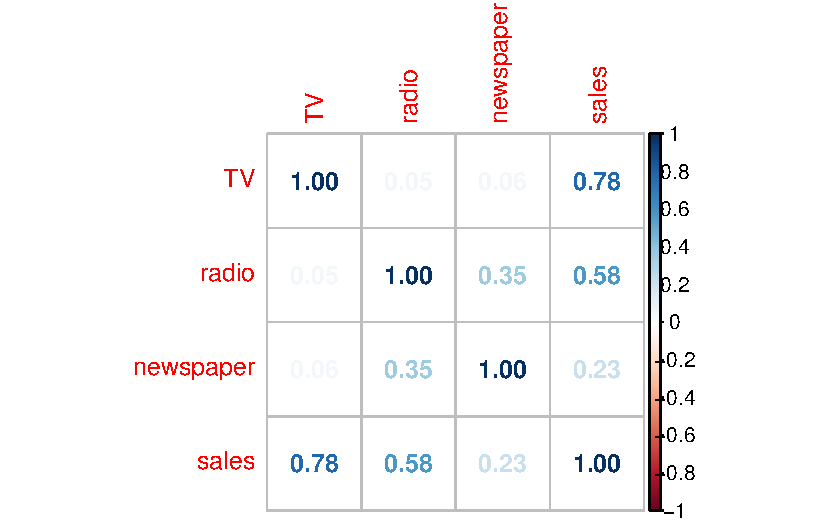
\includegraphics{Chapter3_files/figure-pdf/unnamed-chunk-57-1.pdf}

}

\end{figure}

Notice that correlation between radio and newspaper is 0.35. This
reveals a tendency to spend more on newspaper advertising in markets
where more is spent on radio advertising. Now suppose the multiple
regression is correct and newspaper advertising has no direct impact on
sales, but radio advertising does increase sales. Then in markets where
we spend more on radio, our sales will tend to be higher, adn as our
correaltion matrix shows, we also tend to spend more on newspaper
advertising in those same markets. Hence, in a simple linaer regresion
which only examines sales vs newspaper, we will observe that higher
values of newspaper tend to be associated with higher values of sales,
even though newspaper advertising does not actually affect sales. So
newspaper sales are proxy for radio advertising; newspaper gets credit
for the effect of radio on sales.

This is a very common issue. Consider running a regression of shark
attack versus ice cream sales for data collected at a given beach
community. We would see a positive relationship, similar to that seen
between sales and newspaper. Of course ice creams doesnt cause shark
attacks. In reality higher temperatures cause more people to visit the
beach in trun results in more ice cream sales and more shark attacks. A
multiple regression of attacks versus ice cream sales and temperature
revals that, the former predictr is no longer significant after
adjusting for temperature.

\hypertarget{some-important-questions}{%
\subsection{Some important Questions}\label{some-important-questions}}

When we perform MLR, we usually are interested answering a few important
questions

\begin{enumerate}
\def\labelenumi{\arabic{enumi}.}
\item
  \emph{Is at least one of the predictors} \(x_1, x_2, \dots, x_p\)
  \emph{useful in predicting the response?}
\item
  \emph{Do all predictors help to explain} \(Y\), \emph{or is only a
  subset of the predictors useful?}
\item
  \emph{How well does the model fit the data?}
\end{enumerate}

4 \emph{Given a set of predictor values, what response value should we
predict, and how accurate is our prediction?}

Lets answer these questions:

\begin{enumerate}
\def\labelenumi{\arabic{enumi}.}
\item
  \emph{Is at least one of the predictors} \(x_1, x_2, \dots, x_p\)
  \emph{useful in predicting the response?}

  In SLR we simply checked whether \(\beta_1 = 0\) or not. In MLR, we
  need to ask whether all of the regression coefficients are zero
  \(\beta_1 = \beta_2 = \dots = \beta_p = 0\). So our null hypothesis is

  \[
   \begin{align}
   H_0 &: \beta_1 = \beta_2 = \dots = \beta_o = 0 \\
   H_\alpha &: \text{at least one} \space B_j \space \text{is non-zero}
   \end{align}
   \] This hypothesis test is performed by computing the
  \emph{F-statistic},

  \[
   F = \frac{(TSS - RSS)/p}{RSS/(n-p-1)}
   \] (3.23)

  So, if there is no relationship between the resposne and predictors,
  we expect F-statistic to take on value close to 1. if \(H_\alpha\) is
  true then \(F\) should be greater than 1.
\end{enumerate}

\begin{Shaded}
\begin{Highlighting}[]
\FunctionTok{summary}\NormalTok{(}\FunctionTok{lm}\NormalTok{(sales }\SpecialCharTok{\textasciitilde{}}\NormalTok{ TV }\SpecialCharTok{+}\NormalTok{ radio }\SpecialCharTok{+}\NormalTok{ newspaper, advertising))}
\end{Highlighting}
\end{Shaded}

\begin{verbatim}

Call:
lm(formula = sales ~ TV + radio + newspaper, data = advertising)

Residuals:
    Min      1Q  Median      3Q     Max 
-8.8277 -0.8908  0.2418  1.1893  2.8292 

Coefficients:
             Estimate Std. Error t value Pr(>|t|)    
(Intercept)  2.938889   0.311908   9.422   <2e-16 ***
TV           0.045765   0.001395  32.809   <2e-16 ***
radio        0.188530   0.008611  21.893   <2e-16 ***
newspaper   -0.001037   0.005871  -0.177     0.86    
---
Signif. codes:  0 '***' 0.001 '**' 0.01 '*' 0.05 '.' 0.1 ' ' 1

Residual standard error: 1.686 on 196 degrees of freedom
Multiple R-squared:  0.8972,    Adjusted R-squared:  0.8956 
F-statistic: 570.3 on 3 and 196 DF,  p-value: < 2.2e-16
\end{verbatim}

F statistic is 570 and is far from 1. But it is best to have a look at
the p-value of the F statistic which is also very small.

This means that at least one of the media is associated with increase
sales.

In (3.23) we are testing \(H_0\) that all the coefficients are zero.
Sometimes we want to test that a particular subset of \(q\) of the
coefficients are zero. This corresponesd to a null hypothesis

\[
  H_0 : \beta_{p-q+1} = \beta_{p-q+2} = \dots = \beta_p
  \]

In this case we fit a second model that uses all the variables
\emph{except} those last \(q\). suppose that residual sum of squares for
that model is \(RSS_0\). Then the appropriate F-statistic is

\[
  F = \frac{(RSS_0 - RSS)/q}{RSS/(n-p-1)}
  \] (3.24)

On advertising MLR we saw that newspaper is not significant from its p
value. Then why do we need to look at the overall F-statistic? after
all, it seems likely that if any one of the p-values for the individual
variables is very small, then \emph{at least one of the predictors is
realted to the respose}. This is not true usually, especially when \(p\)
is large.

So after estimating the model first look at the F-statistic, than to the
individual t statistic p values.

\begin{enumerate}
\def\labelenumi{\arabic{enumi}.}
\setcounter{enumi}{1}
\item
  \emph{Do all predictors help to explain} \(Y\), \emph{or is only a
  subset of the predictors useful?} =\textgreater{} \textbf{Deciding on
  important variables}

  After lookig at the F statistic, we can look at the individual p
  values. But if *p\$ is large, we are going to make false discoveries.

  Usually not all predictors are associated with the response. This task
  of determining which predictors are associated with the response in
  order to fit a single model involving only those predictors is refered
  to as \emph{variable selection}. Check out Chapter 6 for more detail.
  But here is a breif outline of some of the classical approaches.

  Ideally we want to perform variable selection by trying out a lot of
  different models, each containing different subset of the predictors.
  For instance if our \(p=2\) then we can consider four models

  \begin{itemize}
  \item
    \begin{enumerate}
    \def\labelenumii{(\arabic{enumii})}
    \tightlist
    \item
      a model containing no variables
    \end{enumerate}
  \item
    \begin{enumerate}
    \def\labelenumii{(\arabic{enumii})}
    \setcounter{enumii}{1}
    \tightlist
    \item
      a model containing \(x_1\) only
    \end{enumerate}
  \item
    \begin{enumerate}
    \def\labelenumii{(\arabic{enumii})}
    \setcounter{enumii}{2}
    \tightlist
    \item
      a model containnig \(x_2\) only
    \end{enumerate}
  \item
    \begin{enumerate}
    \def\labelenumii{(\arabic{enumii})}
    \setcounter{enumii}{3}
    \tightlist
    \item
      a model containing \(x1\) and \(x_2\).
    \end{enumerate}
  \end{itemize}

  We can then select the \emph{best} model out of all the models by
  looking at some statistics we can use to judge the quality of the
  model. These are

  \begin{itemize}
  \tightlist
  \item
    \emph{Mallow}'s \(C_p\)
  \item
    \emph{Akaike information creterion} (AIC)
  \item
    \emph{Bayesian information criterion}(BIC)
  \item
    \emph{adjusted} \(R^2\)
  \end{itemize}

  These are discussed in more detail in chapter 6.

  We can also determine which model is the best by plotting various
  model outputs, such as the residuals, in order to search for patterns.

  But we cannot consider all models, especially when \(p\) is high.
  There are three classical approaches for this task:

  \begin{itemize}
  \tightlist
  \item
    \emph{Forward selection}

    \begin{itemize}
    \item
      begin with \emph{null model} a model that contains an intercept
      but no predictors.
    \item
      Then fit \emph{p} simple linear regressions and add to the null
      model the variable that results in the lowest RSS.
    \item
      Then add to that model the variable that results in the lowest RSS
      for the new two-variable model. This approach is continued until
      some stopping rule is satisfied.
    \end{itemize}
  \item
    \emph{Backward selection}

    \begin{itemize}
    \tightlist
    \item
      Put all varaibles in the model.
    \item
      remove the least statistically significant predictor.
    \item
      estimate the new regression with \(p-1\) variable, remove the
      largest p-value predictor. This procedure continues until a
      stopping rule is reached =\textgreater{} stop after all remaining
      variables have p value \textless{} 0.02
    \end{itemize}
  \item
    \emph{Mixed selection}

    \begin{itemize}
    \tightlist
    \item
      Combination of forward selection and backward selection
    \item
      Start with no variables in the model
    \item
      add the varaible that provides the best fit
    \item
      add varaibles one-by-one
    \item
      at one point if the p-value for one of the variables in the model
      rises above a certain treshold, then we remove that variabel from
      the model.
    \item
      Continue untill all variables have sufficiently low p value, and
      all vairables in the model woudl have a large p-value if added to
      the model
    \end{itemize}
  \end{itemize}

  Backwar slecetion cannot be used if \(p>n\), forward selection can
  always be used.
\item
  \emph{How well does the model fit the data?} \textbf{Model Fit}
\end{enumerate}

Two of the most common numerical measures of model fit are RSE and
\(R^2\).

In SLR \(R^2\) is equal to \(cor(Y,X)\). In MLR
\(R^2 = cor(Y,\hat{Y})\).

\(R^2\) will always increase as you add more variable, even though that
varaible is not statistically significant. This is because adding
another variable must allow us to fit the trainig data(not necessarly
test data) more accurately. But this increase in \(R^2\) after adding a
statistically not-significant varible is very low =\textgreater{}
evidence that you can drop the not significant variable. Check out the
\(R^2\) variables of the following models

\begin{Shaded}
\begin{Highlighting}[]
\FunctionTok{summary}\NormalTok{(}\FunctionTok{lm}\NormalTok{(sales }\SpecialCharTok{\textasciitilde{}}\NormalTok{ TV }\SpecialCharTok{+}\NormalTok{ radio }\SpecialCharTok{+}\NormalTok{ newspaper, advertising))}
\end{Highlighting}
\end{Shaded}

\begin{verbatim}

Call:
lm(formula = sales ~ TV + radio + newspaper, data = advertising)

Residuals:
    Min      1Q  Median      3Q     Max 
-8.8277 -0.8908  0.2418  1.1893  2.8292 

Coefficients:
             Estimate Std. Error t value Pr(>|t|)    
(Intercept)  2.938889   0.311908   9.422   <2e-16 ***
TV           0.045765   0.001395  32.809   <2e-16 ***
radio        0.188530   0.008611  21.893   <2e-16 ***
newspaper   -0.001037   0.005871  -0.177     0.86    
---
Signif. codes:  0 '***' 0.001 '**' 0.01 '*' 0.05 '.' 0.1 ' ' 1

Residual standard error: 1.686 on 196 degrees of freedom
Multiple R-squared:  0.8972,    Adjusted R-squared:  0.8956 
F-statistic: 570.3 on 3 and 196 DF,  p-value: < 2.2e-16
\end{verbatim}

\begin{Shaded}
\begin{Highlighting}[]
\FunctionTok{summary}\NormalTok{(}\FunctionTok{lm}\NormalTok{(sales }\SpecialCharTok{\textasciitilde{}}\NormalTok{ TV }\SpecialCharTok{+}\NormalTok{ radio, advertising))}
\end{Highlighting}
\end{Shaded}

\begin{verbatim}

Call:
lm(formula = sales ~ TV + radio, data = advertising)

Residuals:
    Min      1Q  Median      3Q     Max 
-8.7977 -0.8752  0.2422  1.1708  2.8328 

Coefficients:
            Estimate Std. Error t value Pr(>|t|)    
(Intercept)  2.92110    0.29449   9.919   <2e-16 ***
TV           0.04575    0.00139  32.909   <2e-16 ***
radio        0.18799    0.00804  23.382   <2e-16 ***
---
Signif. codes:  0 '***' 0.001 '**' 0.01 '*' 0.05 '.' 0.1 ' ' 1

Residual standard error: 1.681 on 197 degrees of freedom
Multiple R-squared:  0.8972,    Adjusted R-squared:  0.8962 
F-statistic: 859.6 on 2 and 197 DF,  p-value: < 2.2e-16
\end{verbatim}

They are almost the same.

But lets see the \(R^2\) of the model containing only Tv

\begin{Shaded}
\begin{Highlighting}[]
\FunctionTok{summary}\NormalTok{(}\FunctionTok{lm}\NormalTok{(sales }\SpecialCharTok{\textasciitilde{}}\NormalTok{ TV, advertising))}
\end{Highlighting}
\end{Shaded}

\begin{verbatim}

Call:
lm(formula = sales ~ TV, data = advertising)

Residuals:
    Min      1Q  Median      3Q     Max 
-8.3860 -1.9545 -0.1913  2.0671  7.2124 

Coefficients:
            Estimate Std. Error t value Pr(>|t|)    
(Intercept) 7.032594   0.457843   15.36   <2e-16 ***
TV          0.047537   0.002691   17.67   <2e-16 ***
---
Signif. codes:  0 '***' 0.001 '**' 0.01 '*' 0.05 '.' 0.1 ' ' 1

Residual standard error: 3.259 on 198 degrees of freedom
Multiple R-squared:  0.6119,    Adjusted R-squared:  0.6099 
F-statistic: 312.1 on 1 and 198 DF,  p-value: < 2.2e-16
\end{verbatim}

it is 0.611.

If we add radio

\begin{Shaded}
\begin{Highlighting}[]
\FunctionTok{summary}\NormalTok{(}\FunctionTok{lm}\NormalTok{(sales }\SpecialCharTok{\textasciitilde{}}\NormalTok{ TV }\SpecialCharTok{+}\NormalTok{ radio, advertising))}
\end{Highlighting}
\end{Shaded}

\begin{verbatim}

Call:
lm(formula = sales ~ TV + radio, data = advertising)

Residuals:
    Min      1Q  Median      3Q     Max 
-8.7977 -0.8752  0.2422  1.1708  2.8328 

Coefficients:
            Estimate Std. Error t value Pr(>|t|)    
(Intercept)  2.92110    0.29449   9.919   <2e-16 ***
TV           0.04575    0.00139  32.909   <2e-16 ***
radio        0.18799    0.00804  23.382   <2e-16 ***
---
Signif. codes:  0 '***' 0.001 '**' 0.01 '*' 0.05 '.' 0.1 ' ' 1

Residual standard error: 1.681 on 197 degrees of freedom
Multiple R-squared:  0.8972,    Adjusted R-squared:  0.8962 
F-statistic: 859.6 on 2 and 197 DF,  p-value: < 2.2e-16
\end{verbatim}

It increaes dramatically. This implies that model that uses TV and radio
to predict sales is better than only using Tv. also radio is
statistically signifiacnt.

\begin{Shaded}
\begin{Highlighting}[]
\FunctionTok{summary}\NormalTok{(}\FunctionTok{lm}\NormalTok{(sales }\SpecialCharTok{\textasciitilde{}}\NormalTok{ TV }\SpecialCharTok{+}\NormalTok{ newspaper, advertising))}
\end{Highlighting}
\end{Shaded}

\begin{verbatim}

Call:
lm(formula = sales ~ TV + newspaper, data = advertising)

Residuals:
    Min      1Q  Median      3Q     Max 
-8.6231 -1.7346 -0.0948  1.8926  8.4512 

Coefficients:
            Estimate Std. Error t value Pr(>|t|)    
(Intercept) 5.774948   0.525338  10.993  < 2e-16 ***
TV          0.046901   0.002581  18.173  < 2e-16 ***
newspaper   0.044219   0.010174   4.346 2.22e-05 ***
---
Signif. codes:  0 '***' 0.001 '**' 0.01 '*' 0.05 '.' 0.1 ' ' 1

Residual standard error: 3.121 on 197 degrees of freedom
Multiple R-squared:  0.6458,    Adjusted R-squared:  0.6422 
F-statistic: 179.6 on 2 and 197 DF,  p-value: < 2.2e-16
\end{verbatim}

Not with newspaper though.

Or the opposite

\begin{Shaded}
\begin{Highlighting}[]
\FunctionTok{summary}\NormalTok{(}\FunctionTok{lm}\NormalTok{(sales }\SpecialCharTok{\textasciitilde{}}\NormalTok{ radio, advertising))}
\end{Highlighting}
\end{Shaded}

\begin{verbatim}

Call:
lm(formula = sales ~ radio, data = advertising)

Residuals:
     Min       1Q   Median       3Q      Max 
-15.7305  -2.1324   0.7707   2.7775   8.1810 

Coefficients:
            Estimate Std. Error t value Pr(>|t|)    
(Intercept)  9.31164    0.56290  16.542   <2e-16 ***
radio        0.20250    0.02041   9.921   <2e-16 ***
---
Signif. codes:  0 '***' 0.001 '**' 0.01 '*' 0.05 '.' 0.1 ' ' 1

Residual standard error: 4.275 on 198 degrees of freedom
Multiple R-squared:  0.332, Adjusted R-squared:  0.3287 
F-statistic: 98.42 on 1 and 198 DF,  p-value: < 2.2e-16
\end{verbatim}

\begin{Shaded}
\begin{Highlighting}[]
\FunctionTok{summary}\NormalTok{(}\FunctionTok{lm}\NormalTok{(sales}\SpecialCharTok{\textasciitilde{}}\NormalTok{radio}\SpecialCharTok{+}\NormalTok{TV, advertising))}
\end{Highlighting}
\end{Shaded}

\begin{verbatim}

Call:
lm(formula = sales ~ radio + TV, data = advertising)

Residuals:
    Min      1Q  Median      3Q     Max 
-8.7977 -0.8752  0.2422  1.1708  2.8328 

Coefficients:
            Estimate Std. Error t value Pr(>|t|)    
(Intercept)  2.92110    0.29449   9.919   <2e-16 ***
radio        0.18799    0.00804  23.382   <2e-16 ***
TV           0.04575    0.00139  32.909   <2e-16 ***
---
Signif. codes:  0 '***' 0.001 '**' 0.01 '*' 0.05 '.' 0.1 ' ' 1

Residual standard error: 1.681 on 197 degrees of freedom
Multiple R-squared:  0.8972,    Adjusted R-squared:  0.8962 
F-statistic: 859.6 on 2 and 197 DF,  p-value: < 2.2e-16
\end{verbatim}

\begin{Shaded}
\begin{Highlighting}[]
\FunctionTok{summary}\NormalTok{(}\FunctionTok{lm}\NormalTok{(sales }\SpecialCharTok{\textasciitilde{}}\NormalTok{ radio }\SpecialCharTok{+}\NormalTok{ newspaper, advertising))}
\end{Highlighting}
\end{Shaded}

\begin{verbatim}

Call:
lm(formula = sales ~ radio + newspaper, data = advertising)

Residuals:
     Min       1Q   Median       3Q      Max 
-15.5289  -2.1449   0.7315   2.7657   7.9751 

Coefficients:
            Estimate Std. Error t value Pr(>|t|)    
(Intercept) 9.188920   0.627672  14.640   <2e-16 ***
radio       0.199045   0.021870   9.101   <2e-16 ***
newspaper   0.006644   0.014909   0.446    0.656    
---
Signif. codes:  0 '***' 0.001 '**' 0.01 '*' 0.05 '.' 0.1 ' ' 1

Residual standard error: 4.284 on 197 degrees of freedom
Multiple R-squared:  0.3327,    Adjusted R-squared:  0.3259 
F-statistic: 49.11 on 2 and 197 DF,  p-value: < 2.2e-16
\end{verbatim}

What about RSE:

\begin{Shaded}
\begin{Highlighting}[]
\FunctionTok{summary}\NormalTok{(}\FunctionTok{lm}\NormalTok{(sales }\SpecialCharTok{\textasciitilde{}}\NormalTok{ TV }\SpecialCharTok{+}\NormalTok{ radio, advertising))}
\end{Highlighting}
\end{Shaded}

\begin{verbatim}

Call:
lm(formula = sales ~ TV + radio, data = advertising)

Residuals:
    Min      1Q  Median      3Q     Max 
-8.7977 -0.8752  0.2422  1.1708  2.8328 

Coefficients:
            Estimate Std. Error t value Pr(>|t|)    
(Intercept)  2.92110    0.29449   9.919   <2e-16 ***
TV           0.04575    0.00139  32.909   <2e-16 ***
radio        0.18799    0.00804  23.382   <2e-16 ***
---
Signif. codes:  0 '***' 0.001 '**' 0.01 '*' 0.05 '.' 0.1 ' ' 1

Residual standard error: 1.681 on 197 degrees of freedom
Multiple R-squared:  0.8972,    Adjusted R-squared:  0.8962 
F-statistic: 859.6 on 2 and 197 DF,  p-value: < 2.2e-16
\end{verbatim}

\begin{Shaded}
\begin{Highlighting}[]
\FunctionTok{summary}\NormalTok{(}\FunctionTok{lm}\NormalTok{(sales }\SpecialCharTok{\textasciitilde{}}\NormalTok{ TV }\SpecialCharTok{+}\NormalTok{ radio }\SpecialCharTok{+}\NormalTok{ newspaper, advertising))}
\end{Highlighting}
\end{Shaded}

\begin{verbatim}

Call:
lm(formula = sales ~ TV + radio + newspaper, data = advertising)

Residuals:
    Min      1Q  Median      3Q     Max 
-8.8277 -0.8908  0.2418  1.1893  2.8292 

Coefficients:
             Estimate Std. Error t value Pr(>|t|)    
(Intercept)  2.938889   0.311908   9.422   <2e-16 ***
TV           0.045765   0.001395  32.809   <2e-16 ***
radio        0.188530   0.008611  21.893   <2e-16 ***
newspaper   -0.001037   0.005871  -0.177     0.86    
---
Signif. codes:  0 '***' 0.001 '**' 0.01 '*' 0.05 '.' 0.1 ' ' 1

Residual standard error: 1.686 on 196 degrees of freedom
Multiple R-squared:  0.8972,    Adjusted R-squared:  0.8956 
F-statistic: 570.3 on 3 and 196 DF,  p-value: < 2.2e-16
\end{verbatim}

adding newspaper increased the RSE =\textgreater{} no need to add
newspaper. Adding newspaper increases RSE because

\[
RSE = \sqrt{\frac{1}{n-p-1}RSS}
\]

Models with more variables can have higher RSE if the decrease in RSS is
small relative to the increase in \(p\).

So we can look at both the RSE and \(R^2\).



\end{document}
